\section{Construction of the \ddfv meshes} \label{sec:construction_of_the_ddfv_meshes}

\areprendre{
\begin{envide}[Construction maillages]
\begin{enumerate}
    \item Soit une surface $\surflisse$
    \item On place des points sur la surface $\surflisse$
    \item On en déduit un complexe sur la variété
    \item Ce complexe définit le maillage primal, courbe et polyédrique
    \item On calcule les barycentres des mailles primales plates
    \item On projette ces barycentres sur la surface $\surflisse$
    \item Construction des mailles duales (barycentriques):
    \item Projection du milieu des arêtes primales sur $\surflisse$
    \item Arcs passant par les milieux projetés
    \item Les mailles duales sont approchées par $2m$ facettes
\end{enumerate}    
\end{envide}
}

\subsection{Maillages primaux}

\begin{figure}[p]
    \centering
    \input{figures/ddfv_3d.tex}
    \caption{Triangulated surface from the point of view of the differential geometry}
    \label{fig:ddfv_3d}
\end{figure}

Dans la \Cref{sec:hypothesis_on_the_surface_and_projection}, nous avons introduit plusieurs objets géométriques:
\begin{itemize}
    \item la surface lisse $\surflisse$;
    \item le projecteur $\fonctionens[\projvariete]{\surfpoly}{\surflisse}$;
    \item la surface polyédrique $\surfpoly$;
    \item un maillage $\ensprimalplat$ nommé \defini{maillage primal plat}, dont les mailles sont notées $\primalplat{K}$, $\primalplat{L}$ et les arêtes sont notées $\sigma$. 
    \item un maillage $\ensprimal$ nommé \defini{maillage primal courbe}, dont les mailles sont $\primal{K} \defeq \projvariete \primalplat{K}$ et les arêtes sont $\sigmacourbe \defeq \projvariete \sigma$.
\end{itemize}

\begin{equation} \label{eq:surfpoly}
\surfpoly = \bigcup_{\primalplat{K} \in \ensprimalplat} \primalplat{K}, 
\end{equation}
\begin{equation} \label{eq:primalK}
\forall \primalplat{K} \subset \surfpoly, \quad \exists! \primal{K} \defeq \projvariete \primalplat{K} \subset \surflisse.
\end{equation}
The \defini{primal mesh} $\ensprimal$ is the set of disjoint polygonal control volumes $\primal{K}$:
\begin{equation} \label{eq:ensprimal}
    \ensprimal \defeq \ens[\big]{\primal{K} = \projvariete \primalplat{K} \tq \primalplat{K} \in \ensprimalplat}
\end{equation}
\[
\surflisse = \bigcup_{\primal{K} \in \ensprimal} \primal{K}.
\]
We create a representative point $x_{\primalplat{K}}$  of each triangle $\primalplat{K} \in \ensprimalplat$ (\ref{fig:ddfv_3d}, bottom left). The point $x_{\primalplat{K}}$ is taken at the barycenter of triangle $\primalplat{K}$. The denote 
\begin{equation} \label{eq:xprimalK}
x_{\primal{K}} \defeq \projvariete x_{\primalplat{K}}
\end{equation}
its projection onto the smooth surface $\surflisse$. 

We call 
\begin{equation} \label{eq:enssomdualplat}
    \enssomdualplat \defeq 
    \ens[\big]{x_{\primalplat{K}} \tq \primalplat{K} \in \ensprimalplat}
\end{equation}
this family of points and let $\enssomdual$ denote the set of vertices of the \areprendre{mesh $\ensdual$}:
\begin{equation} \label{eq:enssomdual}
    \enssomdual \defeq \ens[\big]{x_{\primal{K}} \tq \primal{K} \in \ensprimal}.
\end{equation}
For all adjacent control volumes $\primalplat{K}$ and $\primalplat{L}$, we assume that $\partial \primalplat{K} \cap \partial \primalplat{L}$ is a segment that we call \defini{an edge of the mesh} $\ensprimalplat$ and that we denote by 
\begin{equation} \label{eq:sigma}
\sigma = \sigma_{\primalplat{K},\primalplat{L}} \defeq \arete{\primalplat{K}}{\primalplat{L}}. 
\end{equation}
Let $\ensareteprimplat$ be the set of such edges. 

\begin{equation} \label{eq:enssomprim_plat}
\enssomprim = \ens[\big]{x_{\mailleduale{K}} \tq \mailleduale{K} \in \ensdual}
=
\enssomprimplat = \ens[\big]{x_{\mailledualeplate{K}} \tq \mailledualeplate{K} \in \ensdualplat}
\end{equation}
\[
x_{\mailledualeplate{K}} = x_{\mailleduale{K}}
\]


\begin{equation} \label{eq:sigmacourbe}
    \forall \sigma \in \ensareteprimplat, \quad \sigmacourbe \defeq \projvariete \sigma
\end{equation}

\areprendre{citation à ajouter}

For all bounded set $E \subset \R^d$, set the \defini{diameter}
\begin{equation} \label{eq:diamE}
\diam{E} \defeq \sup\limits_{x,y \in E} \abs{x - y}.
\end{equation}

We denote by $\mesure(E)$ the measure of an object $E$ in its natural dimension (i.e. the $d$-dimensional measure, if $E$ is a control volume, a dual control volume or a diamond; and the $(d - 1)$-dimensional measure, if $E$ is an interface or a part of an interface). 

\noindent For any control volume $\primal{K} \in \ensprimal$, we define
\areprendre{
\begin{itemize}
    \item $\mesure(\primal{K})$, the measure of $\primal{K}$;
    \item $\ensareteprim_{\primal{K}}$, the set of edges of $\primal{K}$;
    \item $\ensdiamant_{\primal{K}} = \ens[\big]{\diamant{D}_{\sigma, \dual{\sigma}} \in \ensdiamant \tq \sigma \in \ensareteprim_{\primal{K}}}$;
    \item $\vect{\nu}_{\primal{K}}$, the outward unit normal vector to $\partial \primal{K}$;
    \item $\diam{\primal{K}}$, the diameter of $\primal{K}$.
\end{itemize}
}

\areprendre{
It can happen that the point $x_{\primal{K}}$ does not belong to $\primal{K}$ (if $\primal{K}$ is a triangle and $x_{\primal{K}}$ its circumcenter for instance). As usual in that case (see \cite{eymard_finite_2000}) it is necessary to assume that $\vect{\nu}_{\primal{K}}$ points from $x_{\primal{K}}$ towards $x_{\primal{L}}$, that is $\vect{\nu}_{\primal{K}} = \vect{\nu}$ with the notations above. Similarly we assume that $\vect{\nu}_{\mailleduale{K}} = \dual{\vect{\nu}}$. In the case of a triangular mesh $\ensprimal$ in which $x_{\primal{K}}$ is the circumcenter of $\primal{K}$, this assumption is known as the Delaunay condition. 
}

\subsection{Dual mesh (Maillage dual barycentrique)}

\begin{figure}[H]
    \centering
    \tikzset{
    ddfv/.style={
        scale=1.5,
        every path/.style={thick,line join=round, cap=round},
        ptsq/.style 2 args={
          rectangle,
          fill=##1,
          inner sep=2pt,
          label={[text=##1]##2}
        },
        ptsqbord/.style 2 args={
          rectangle,
          draw=##1,
          inner sep=2pt,
          label={[text=##1]##2}
        },
        ptcl/.style 2 args={
          circle,
          fill=##1,
          inner sep=1.5pt,
          label={[text=##1]##2}
        },
        ptclbord/.style 2 args={
          circle,
          draw=##1,
          inner sep=1.5pt,
          label={[text=##1]##2}
        },
        mailleprimale/.style={
            myblue,
            fill=mylightblue
        },
        mailledualeint/.style={
            myred,
            fill=mylightred
        },
        mailledualebord/.style={
            myred,
            fill=mylightred!50!white
        },
        maillediamantint/.style={
            mygreen,
            fill=mylightgreen
        },
        maillediamantbord/.style={
            mygreen,
            fill=mylightgreen!50!white
        }
    }
}

\def\Rayon{2}
\def\xzero{0}
\def\yzero{0}
\def\zzero{0}

\makeatletter

\newcommand{\PointXYZ}[4]{%
    \pgfmathsetmacro{\px}{#2}%
    \pgfmathsetmacro{\py}{#3}%
    \pgfmathsetmacro{\pz}{#4}%
    \coordinate (#1) at (\px,\py,\pz);
    \expandafter\xdef\csname pt@#1@x\endcsname{\px}%
    \expandafter\xdef\csname pt@#1@y\endcsname{\py}%
    \expandafter\xdef\csname pt@#1@z\endcsname{\pz}%
}

\newcommand{\GetX}[1]{\csname pt@#1@x\endcsname}
\newcommand{\GetY}[1]{\csname pt@#1@y\endcsname}
\newcommand{\GetZ}[1]{\csname pt@#1@z\endcsname}

\newcommand{\MidPointXYZ}[3]{%
    \pgfmathsetmacro{\mx}{0.5*(\GetX{#2}+\GetX{#3})}%
    \pgfmathsetmacro{\my}{0.5*(\GetY{#2}+\GetY{#3})}%
    \pgfmathsetmacro{\mz}{0.5*(\GetZ{#2}+\GetZ{#3})}%
    \PointXYZ{#1}{\mx}{\my}{\mz}%
}

\makeatother

\pgfmathdeclarefunction{f}{2}{%
  \pgfmathparse{\zzero + sqrt(max(0,\Rayon^2-(#1-\xzero)^2-(#2-\yzero)^2))}%
}

\tdplotsetmaincoords{45}{55}

\begin{tikzpicture}[
    scale=1.5,
    node distance=0.6cm,
    every node/.style={inner sep=0pt},
    ddfv,
    tdplot_main_coords,
    angle eccentricity=1.35,
    angle radius=7mm,
]

\coordinate (O) at (0,0,0);
\PointXYZ{fO}{0}{0}{f(0,0)};

\def\Rpenta{1.5}

\foreach \i/\j/\angleA/\angleB in {
    1/2/13/17,
    2/3/17/21,
    3/4/21/5,
    4/5/5/9,
    5/1/9/13
}
{
    % Point F_i
    \pgfmathsetmacro{\xA}{\Rpenta*cos((\angleA*pi/10)r)}
    \pgfmathsetmacro{\yA}{\Rpenta*sin((\angleA*pi/10)r)}
    \pgfmathsetmacro{\zA}{f(\xA,\yA)}

    \PointXYZ{F\i}{\xA}{\yA}{0};
    % \coordinate (fF\i) at ({\xA},{\yA},{\zA});
    \PointXYZ{fF\i}{\xA}{\yA}{\zA};

    % \node[ptsq={myblue}{}] at (F\i) {};
    % \node[ptsq={myblue}{}] at (fF\i) {};

    % Point F_j
    \pgfmathsetmacro{\xB}{\Rpenta*cos((\angleB*pi/10)r)}
    \pgfmathsetmacro{\yB}{\Rpenta*sin((\angleB*pi/10)r)}
    \pgfmathsetmacro{\zB}{f(\xB,\yB)}

    \coordinate (F\j)  at ({\xB},{\yB},0);
    \coordinate (fF\j) at ({\xB},{\yB},{\zB});

    % Barycentre euclidien du triangle fO, fF_i, fF_j
    \pgfmathsetmacro{\xG}{(\xzero+\xA+\xB)/3}
    \pgfmathsetmacro{\yG}{(\yzero+\yA+\yB)/3}
    \pgfmathsetmacro{\zG}{(f(0,0)+f(\xA,\yA)+f(\xB,\yB))/3}

    % Projection radiale sur la sphère de centre (xzero,yzero,zzero)
    \pgfmathsetmacro{\normG}{
        sqrt((\xG-\xzero)^2 + (\yG-\yzero)^2 + (\zG-\zzero)^2)
    }

    \pgfmathsetmacro{\xProjG}{\xzero + 1.2*\Rayon*(\xG-\xzero)/\normG}
    \pgfmathsetmacro{\yProjG}{\yzero + 1.2*\Rayon*(\yG-\yzero)/\normG}
    \pgfmathsetmacro{\zProjG}{\zzero + 1.2*\Rayon*(\zG-\zzero)/\normG}

    % \coordinate (fG\i) at ({\xProjG},{\yProjG},{\zProjG});
    \PointXYZ{fG\i}{\xProjG}{\yProjG}{\zProjG};

    %%%%%%%%%%%%%%%%%%%%%%%%%%%%%%%%%%%%%%%%%%%%%%%%%%%%%%%%%%%%%%%%%%%

    \pgfmathsetmacro{\xG}{(\xA+\xB)/3}
    \pgfmathsetmacro{\yG}{(\yA+\yB)/3}
    \pgfmathsetmacro{\zG}{(f(0,0)+f(\xA,\yA)+f(\xB,\yB))/3}

    \coordinate (G\i) at ({\xG},{\yG},{\zG});

    \MidPointXYZ{M\i}{fO}{fF\i}
}
    
\draw[myblue] (fF1) -- (fF2) -- (fF3) -- (fF4) -- (fF5) -- cycle;
\draw[mailledualeint] (M1) -- (G1) -- (M2) -- (G2) -- (M3) -- (G3) -- (M4) -- (G4) -- (M5) -- (G5) -- cycle;

\foreach \i in {1,...,5} {
    \draw[myblue] (fO) -- (fF\i);
}

\foreach \i in {1,2,3,4,5}
{
    \draw (G\i) -- (fO);
    \draw[dashed, thin] (G\i) -- (fG\i);
    \node[ptcl={myred}{}] at (G\i) {};
    \node[ptcl={myred}{}] at (fG\i) {};
    \node[ptsq={black}{}] at (M\i) {};
}

\node[ptsq={myblue}{}] at (fO) {};

\foreach \i in {1,2,3,4,5}
{
    \node[ptsq={myblue}{}] at (fF\i) {};
}

\node[myblue, above=6pt] at (fO) {\contour{mylightred!50!white}{$x_{\mailledualeplate{K}}$}};
\node[above=5pt] at (M2) {\contour{mylightred!50!white}{$x_\sigma$}};
\node[myblue] at ($(fO)!0.8!(fF2)$) {\contour{white}{$\sigma_{\primalplat{K},\primalplat{L}}$}};
\node[myred, below=5pt] at (G1) {$x_{\primalplat{L}}$};
\node[myred, above=5pt] at (fG1) {\contour{white}{$x_{\primal{L}}$}};
\node[myred, below=5pt] at (G2) {$x_{\primalplat{K}}$};
\node[myred, above=5pt] at (fG2) {$x_{\primal{K}}$};
\node[myblue, left=5pt] at ($(fF1)!0.5!(fF2)$) {$\primalplat{L}$};
\node[myblue, below=5pt] at ($(fF2)!0.5!(fF3)$) {$\primalplat{K}$};
\node[myred, below=5pt] at ($(G2)!0.5!(M2)$) {$\mailledualeplate{K}$};

\begin{comment}
\pic[
    draw,
    ->,
    "$\theta_i$"
] {angle=G1--fO--M2};

\pic[
    draw,
    ->,
    "$\theta'_i$"
] {angle=M2--fO--G2};
\end{comment}

% Point d'extension pour les variantes de cette figure.
\ifdefined\DecoupageDualPlatExtra
    \DecoupageDualPlatExtra
\fi

\end{tikzpicture}

    \caption{Maille duale plate $\mailledualeplate{K}$}
    \label{fig:decoupage_dual_plat_def}
\end{figure}

\areprendre{
The set $\ensdualplat$ is a family of \chevron{dual} control volumes defined as follows. To any point $x_{\mailleduale{K}} \in \enssomdual$, we associate the \chevron{polygon} $\mailledualeplate{K} \in \ensdualplat$ whose vertices are 
\begin{equation} \label{eq:mailledualeplate}
\ens[\big]{x_{\primal{K}} \in \enssomprim \tq x_{\mailleduale{K}} \in \overline{\primal{K}}, \primal{K} \in \ensprimal}
\end{equation}
sorted with respect to the clockwise order of the corresponding primal control volumes.

The corresponding notations $\dual{\sigma} = \arete{\mailleduale{K}}{\mailleduale{L}}$ and $\ensaretedual$ refer to the dual mesh $\ensdual$.

The finite volume mesh is constructed by the barycentric subdivision of $\surflisse$. The finite volume (or covolume) {\color{red}$V_i$} $\mailleduale{K} \in \ensdual$ around a vertex {\color{red}$X_i$} $x_{\mailleduale{K}}$ is a region bounded by the piecewise linear curve joining the barycenters of the neighbouring triangles and the midpoints of the edges leading to the neighbouring vertices $X_{i,p}$, $p \in \intervalleentier{1}{m}$ where $m$ is the number of neighbours.
}



In the same way, for a dual control volume $\mailleduale{K} \in \ensdual$, we set
\begin{itemize}
    \item $\mesure(\mailleduale{K})$, the measure of $\mailleduale{K}$;
    \item $\ensareteprim_{\mailleduale{K}}$, the set of edges of $\mailleduale{K}$;
    \item $\ensdiamant_{\mailleduale{K}} = \ens[\big]{\diamant{D}_{\sigma, \dual{\sigma}} \in \ensdiamant \tq \dual{\sigma} \in \ensareteprim_{\mailleduale{K}}}$;
    \item $\vect{\nu}_{\mailleduale{K}}$, the outward unit normal vector to $\partial \mailleduale{K}$;
    \item $\diam{\mailleduale{K}}$, the diameter of $\mailleduale{K}$. 
\end{itemize}

\subsection{Diamond mesh} \label{subsec:diamond_set}

Next, we construct a flat diamond set as follows. We consider a couple $(\sigma, \dual{\sigma}) \in \ensareteprimplat \times \ensaretedualplat$ such that $\sigma = \arete{\primalplat{K}}{\primalplat{L}}$ and $\dual{\sigma} = \segment{x_{\primal{K}}}{x_{\primal{L}}}$. We denote by $x_{\mailleduale{K}}$ and $x_{\mailleduale{L}}$ the endpoints of the edge $\sigma$. We consider the plane $P_{\sigma, \dual{\sigma}}$ passing through the midpoints of the segments $\segment{x_{\primal{K}}}{x_{\mailleduale{K}}}$, $\segment{x_{\primal{K}}}{x_{\mailleduale{L}}}$, $\segment{x_{\primal{L}}}{x_{\mailleduale{L}}}$ and $\segment{x_{\primal{L}}}{x_{\mailleduale{K}}}$. This choice makes the construction of the plane easier but is arbitrary. The main thing is that the plan $P_{\sigma, \dual{\sigma}}$ is the one defined by the segments $\sigma$ and $\dual{\sigma}$. We then define the quadrilateral diamond cell $\diamantplat{D}_{\sigma, \dual{\sigma}}$ whose vertices are the projections of the points $x_{\primal{K}}$, $x_{\primal{L}}$, $x_{\mailleduale{K}}$ and $x_{\mailleduale{L}}$ onto the plane $P_{\sigma, \dual{\sigma}}$ in the direction of the vector $\sigma \times \dual{\sigma}$ (\Cref{fig:ddfv_3d_diamant}). By abuse of notation, we still denote by $\sigma$ and $\dual{\sigma}$ the diagonals of the flat diamond cell $\diamantplat{D}_{\sigma, \dual{\sigma}}$. A flat diamond is also illustrated on \ref{fig:ddfv_3d}, bottom left. 
\areprendre{Notice that the flat diamond cells are the union of two disjoint triangles and can be non convex.} The set of flat diamond cells is denoted by $\ensdiamantplat$. Our diamond set is a generalization of 2D planar diamond set used in \ddfv method developed in \cite{domelevo_finite_2005} to 2D surfaces in $\R^3$. 

\bigskip

For all adjacent control volumes $\primalplat{K}$ and $\primalplat{L}$, we denote by 
\begin{equation} \label{eq:dual_sigma}
\dual{\sigma} \defeq \segment{x_{\primal{K}}}{x_{\primal{L}}}
\end{equation}
the segment joining the projections of their representative points. Let $\ensaretedualplat$ be the set of such segments.

On note $\side$ un côté d'un diamant plat $\diamantplat{D}$ et $\ensareteprimplat_{\diamantplat{D}}$ l'ensemble de ses côtés. 

\begin{equation} \label{eq:sidecourbe}
    \sidecourbe \defeq \projvariete \side.
\end{equation}

\begin{figure}[H]
\centering
\begin{subfigure}[c]{.5\textwidth}
    \centering
    \tikzset{
    ddfv/.style={
        scale=1.5,
        every path/.style={thick,line join=round, cap=round},
        ptsq/.style 2 args={
          rectangle,
          fill=##1,
          inner sep=2pt,
          label={[text=##1]##2}
        },
        ptsqbord/.style 2 args={
          rectangle,
          draw=##1,
          inner sep=2pt,
          label={[text=##1]##2}
        },
        ptcl/.style 2 args={
          circle,
          fill=##1,
          inner sep=1.5pt,
          label={[text=##1]##2}
        },
        ptclbord/.style 2 args={
          circle,
          draw=##1,
          inner sep=1.5pt,
          label={[text=##1]##2}
        },
        mailleprimale/.style={
            myblue,
            fill=mylightblue
        },
        mailledualeint/.style={
            myred,
            fill=mylightred
        },
        mailledualebord/.style={
            myred,
            fill=mylightred!50!white
        },
        maillediamantint/.style={
            mygreen,
            fill=mylightgreen
        },
        maillediamantbord/.style={
            mygreen,
            fill=mylightgreen!50!white
        }
    }
}

\makeatletter

\newcommand{\PointXYZ}[4]{%
    \pgfmathsetmacro{\px}{#2}%
    \pgfmathsetmacro{\py}{#3}%
    \pgfmathsetmacro{\pz}{#4}%
    \coordinate (#1) at (\px,\py,\pz);
    \expandafter\xdef\csname pt@#1@x\endcsname{\px}%
    \expandafter\xdef\csname pt@#1@y\endcsname{\py}%
    \expandafter\xdef\csname pt@#1@z\endcsname{\pz}%
}

\newcommand{\GetX}[1]{\csname pt@#1@x\endcsname}
\newcommand{\GetY}[1]{\csname pt@#1@y\endcsname}
\newcommand{\GetZ}[1]{\csname pt@#1@z\endcsname}

\newcommand{\MidPointXYZ}[3]{%
    \pgfmathsetmacro{\mx}{0.5*(\GetX{#2}+\GetX{#3})}%
    \pgfmathsetmacro{\my}{0.5*(\GetY{#2}+\GetY{#3})}%
    \pgfmathsetmacro{\mz}{0.5*(\GetZ{#2}+\GetZ{#3})}%
    \PointXYZ{#1}{\mx}{\my}{\mz}%
}

\newcommand{\LinePlaneIntersection}[6]{%
    \pgfmathsetmacro{\ux}{\GetX{#5}-\GetX{#4}}%
    \pgfmathsetmacro{\uy}{\GetY{#5}-\GetY{#4}}%
    \pgfmathsetmacro{\uz}{\GetZ{#5}-\GetZ{#4}}%

    \pgfmathsetmacro{\vx}{\GetX{#6}-\GetX{#4}}%
    \pgfmathsetmacro{\vy}{\GetY{#6}-\GetY{#4}}%
    \pgfmathsetmacro{\vz}{\GetZ{#6}-\GetZ{#4}}%

    \pgfmathsetmacro{\nx}{\uy*\vz-\uz*\vy}%
    \pgfmathsetmacro{\ny}{\uz*\vx-\ux*\vz}%
    \pgfmathsetmacro{\nz}{\ux*\vy-\uy*\vx}%

    \pgfmathsetmacro{\dx}{\GetX{#3}-\GetX{#2}}%
    \pgfmathsetmacro{\dy}{\GetY{#3}-\GetY{#2}}%
    \pgfmathsetmacro{\dz}{\GetZ{#3}-\GetZ{#2}}%

    \pgfmathsetmacro{\den}{\nx*\dx+\ny*\dy+\nz*\dz}%
    \pgfmathsetmacro{\num}{\nx*(\GetX{#4}-\GetX{#2})+\ny*(\GetY{#4}-\GetY{#2})+\nz*(\GetZ{#4}-\GetZ{#2})}%

    \pgfmathsetmacro{\tt}{\num/\den}%

    \pgfmathsetmacro{\ix}{\GetX{#2}+\tt*\dx}%
    \pgfmathsetmacro{\iy}{\GetY{#2}+\tt*\dy}%
    \pgfmathsetmacro{\iz}{\GetZ{#2}+\tt*\dz}%

    \PointXYZ{#1}{\ix}{\iy}{\iz}%
}

\makeatother

\tdplotsetmaincoords{40}{-105} % élévation, azimut

\begin{tikzpicture}[
    ddfv,
    tdplot_main_coords,
    scale=3.5,
]

\def\a{0.2}

\PointXYZ{xke}{0}{0.5}{0}
\PointXYZ{xle}{0}{-0.5}{0}
\PointXYZ{xk}{-0.25}{0}{0}
\PointXYZ{xl}{0.25}{0}{0}

\PointXYZ{xkez}{0}{0.5}{0.5} % 0.5
\PointXYZ{xlez}{0}{-0.5}{0.5} % 1.3
\PointXYZ{xkz}{-0.25}{0}{1.2} % 1.2
\PointXYZ{xlz}{0.25}{0}{1.2} % 1.3

\MidPointXYZ{xlezxkz}{xlez}{xkz}
\MidPointXYZ{xlezxlz}{xlez}{xlz}
\MidPointXYZ{xkezxkz}{xkez}{xkz}
\MidPointXYZ{xkezxlz}{xkez}{xlz}

\LinePlaneIntersection{I}{xle}{xlez}{xlezxkz}{xlezxlz}{xkezxlz}
\LinePlaneIntersection{J}{xl}{xlz}{xlezxkz}{xlezxlz}{xkezxlz}
\LinePlaneIntersection{K}{xke}{xkez}{xlezxkz}{xlezxlz}{xkezxlz}
\LinePlaneIntersection{L}{xk}{xkz}{xlezxkz}{xlezxlz}{xkezxlz}

\draw[myblue] (xlez) -- (xkez) node[midway, below] {$\sigma$};

\draw[mygreen] (xlezxkz) -- (xlez);
\draw[mygreen] (xkezxlz) -- (xkez);
\draw[mygreen] (xkezxkz) -- (xkez);
\draw[mygreen] (xlezxlz) -- (xlez);

\draw[dash pattern=on 3pt off 2pt, dash phase=0pt] (xlez) -- (I);
\draw[dash pattern=on 3pt off 2pt, dash phase=0pt, ->] (I) --++(0,10pt) node[above] {${\color{myblue} \sigma} \times {\color{myred} \dual{\sigma}}$};

\draw[dash pattern=on 3pt off 2pt, dash phase=0pt] (xkez) -- (K);

\draw[maillediamantint, opacity=0.8, ultra thick] (xlezxkz) -- (I) -- (xlezxlz) -- (J) -- (xkezxlz) -- (K) -- (xkezxkz) -- (L) -- cycle;

\draw[dash pattern=on 3pt off 2pt, dash phase=0pt] (J) -- (xlz);
\draw[dash pattern=on 3pt off 2pt, dash phase=0pt] (L) -- (xkz);

\draw[myblue, dashed] (I) -- (K);
\draw[myred, dashed] (J) -- (L);

\draw[mygreen] (xlezxkz) -- (xkz);
\draw[mygreen] (xkezxlz) -- (xlz);
\draw[mygreen] (xkezxkz) -- (xkz);
\draw[mygreen] (xlezxlz) -- (xlz);

\draw[dotted] (xlezxkz) -- (xlezxlz) -- (xkezxlz) -- (xkezxkz) -- cycle;

\draw[myred] (xlz) -- (xkz) node[midway, right] {$\dual{\sigma}$};


\node[ptsq={black}{}] at (xlezxkz) {};
\node[ptsq={black}{}] at (xlezxlz) {};
\node[ptsq={black}{}] at (xkezxkz) {};
\node[ptsq={black}{}] at (xkezxlz) {};

% \node[ptsq={black}{right:{\contour{white}{$\displaystyle \frac{x_\primal{L}+x_\dual{K}}{2}$}}}] at (xlezxkz) {};
% \node[ptsq={black}{above:{\contour{white}{$\displaystyle \frac{x_\primal{K}+x_\dual{K}}{2}$}}}] at (xlezxlz) {};
% \node[ptsq={black}{below:{\contour{white}{$\displaystyle\hspace*{4pt}\frac{x_\primal{L}+x_\dual{L}}{2}$}}}] at (xkezxkz) {};
% \node[ptsq={black}{left:{\contour{white}{$\displaystyle \frac{x_\primal{K}+x_\dual{L}}{2}$}}}] at (xkezxlz) {};

\node[ptsq={myblue}{right:{\contour{white}{$x_{\dual{K}}$}}}] at (xlez) {};
\node[ptsq={myblue}{left:{\contour{white}{$x_{\dual{L}}$}}}] at (xkez) {};
\node[ptcl={myred}{above:{\contour{white}{$x_{\primal{K}}$}}}] at (xlz) {};
\node[ptcl={myred}{below right:{\contour{mylightgreen!80!white}{$x_{\primal{L}}$}}}] at (xkz) {};

% \node[ptcl={black}{}] at (I) {};
% \node[ptcl={black}{}] at (J) {};
% \node[ptcl={black}{}] at (K) {};
% \node[ptcl={black}{}] at (L) {};

\MidPointXYZ{proj}{J}{L}
% \node[green] at (proj) {$\diamant{D}_{\sigma,\dual{\sigma}}$};
\node[above left, mygreen] at (xkezxlz) {$\diamant{D}_{\sigma,\dual{\sigma}}$};


\def\eqw{0.8pt}

\coordinate (eqA) at ($(I)!\eqw!(L)$);
\coordinate (eqB) at ($(I)!-\eqw!(xlez)$);
\coordinate (eqC) at ($(eqA)+(eqB)-(I)$);
\coordinate (eqD) at ($(I)!\eqw!(J)$);
\coordinate (eqE) at ($(eqD)+(eqB)-(I)$);

\draw[semithick] (I) -- (eqA) -- (eqC) -- (eqB) -- cycle;
\draw[semithick] (I) -- (eqD) -- (eqE) -- (eqB) -- cycle;

\begin{scope}
    
\def\eps{-0.5pt}
\def\lon{0.3pt}

\coordinate (Mq11) at ($(xkez)!0.5!(xkezxkz) + (-\eps,-\lon)$);
\coordinate (Mq12) at ($(xkez)!0.5!(xkezxkz) + (\eps,\lon)$);

\coordinate (Mq21) at ($(xkezxkz)!0.5!(xkz) + (-\eps,-\lon)$);
\coordinate (Mq22) at ($(xkezxkz)!0.5!(xkz) + (\eps,\lon)$);

\begin{scope}[transform canvas={yshift=0.05cm}]
    \draw (Mq11) -- (Mq12);
    \draw (Mq21) -- (Mq22);
\end{scope}

\begin{scope}[transform canvas={yshift=-0.05cm}]
    \draw (Mq11) -- (Mq12);
    \draw (Mq21) -- (Mq22);
\end{scope}

\end{scope}

\end{tikzpicture}
    \caption{Construction of a diamond}
    \label{fig:ddfv_3d_diamant}
\end{subfigure}%
\begin{subfigure}[c]{.5\textwidth}
    \centering
    \tikzset{
    ddfv/.style={
        scale=1.5,
        every path/.style={thick,line join=round, cap=round},
        ptsq/.style 2 args={
          rectangle,
          fill=##1,
          inner sep=2pt,
          label={[text=##1]##2}
        },
        ptsqbord/.style 2 args={
          rectangle,
          draw=##1,
          inner sep=2pt,
          label={[text=##1]##2}
        },
        ptcl/.style 2 args={
          circle,
          fill=##1,
          inner sep=1.5pt,
          label={[text=##1]##2}
        },
        ptclbord/.style 2 args={
          circle,
          draw=##1,
          inner sep=1.5pt,
          label={[text=##1]##2}
        },
        mailleprimale/.style={
            myblue,
            fill=mylightblue
        },
        mailledualeint/.style={
            myred,
            fill=mylightred
        },
        mailledualebord/.style={
            myred,
            fill=mylightred!50!white
        },
        maillediamantint/.style={
            mygreen,
            fill=mylightgreen
        },
        maillediamantbord/.style={
            mygreen,
            fill=mylightgreen!50!white
        }
    }
}

\begin{tikzpicture}[
  ddfv,
  scale=5,
]

\def\a{0.2}

\coordinate (xke) at (0,0.5);
\coordinate (xle) at (0,-0.5);
\coordinate (xk) at (-0.35,0.4);
\coordinate (xl) at (0.35,0.3);
\coordinate (xm) at ($(xke)!0.5!(xle)$);

\node[ptsq={myblue}{above:{\contour{white}{$x_{\mailleduale{K}}$}}}] at (xke) {};

\node[ptsq={myblue}{below:{\contour{white}{$x_{\mailleduale{L}}$}}}] at (xle) {};

\node[ptcl={myred}{left:{$x_{\primal{K}}$}}] at (xk) {};
\node[ptcl={myred}{right:{$x_{\primal{L}}$}}] at (xl) {};

% \node[left, mygreen] at ($(xk)!0.5!(xke)$) {$\diamant{D}_{\sigma,\dual{\sigma}}$};

\path[name path=sigma] (xle) -- (xke);
\path[name path=sigmae] (xk) -- (xl);

\path[name intersections={of=sigma and sigmae, by=I}];

\def\rayonangle{0.08}

\path let
    \p0 = (I),
    \p1 = (xke),
    \p2 = (xl)
in
    \pgfextra{
        \pgfmathsetmacro{\angA}{atan2(-\y1+\y0,\x1-\x0)}
        \pgfmathsetmacro{\angB}{atan2(\y2-\y0,\x2-\x0)}
        \global\let\angA\angA
        \global\let\angB\angB
    };

\draw[black] ($(I)+(\angA:\rayonangle)$) arc[start angle=\angA,end angle=\angB,radius=\rayonangle];
% \fill[opacity=0.5] (I) -- ($(I)+(\angA:\rayonangle)$) arc[start angle=\angA,end angle=\angB,radius=\rayonangle] -- cycle;

\node[right] at ($(I)+({0.5*(\angA+\angB)}:\rayonangle)$) {$\alpha_{\diamant{D}}$};

\draw[myblue]
    (xle) -- (xke)
    node[pos=0.2, right] {$\sigma$};

\draw[myred]
    (xk) -- (xl)
    node[pos=0.7, above] {$\dual{\sigma}$};

\draw[myred] (xk) -- (xm);
\draw[myred] (xl) -- (xm);
\node[ptsq={black}{right:{$x_{\diamant{D}}$}}] at (xm) {};

\def\lengthbasis{2pt}
\def\lengthsq{0.5pt}

\draw[ultra thick, ->] ($(xke)!0.8!(xle)$) -- ++(0,-\lengthbasis) node[right] {$\vect{\tau}_{\mailleduale{K},\mailleduale{L}}$};
\draw[ultra thick, ->] ($(xke)!0.8!(xle)$) -- ++(\lengthbasis,0) node[above] {$\vect{\nu}_{\sigma \primal{K}}$};
\draw ($(xke)!0.8!(xle)$) rectangle ++(\lengthsq,-\lengthsq);

%%%%%%%%%%%%%%%%%%%%%%%%%

\def\position{0.25}

\draw[ultra thick, ->] ($(xk)!\position!(xl)$) -- ($(xk)!\position!(xl)!\lengthbasis!(xl)$) node[above] {$\vect{\tau}_{\primal{K},\primal{L}}$};
\draw[ultra thick, ->] ($(xk)!\position!(xl)$) -- ($(xk)!\position!(xl)!\lengthbasis!-90:(xl)$) node[right] {$\vect{\nu}_{\dual{\sigma} \mailleduale{K}}$};

\coordinate (P) at ($(xk)!\position!(xl)$);
\draw (P) -- ($(P)!\lengthsq!(xl)$) -- ($(P)!\lengthsq!(xl)!\lengthsq!-90:(xl)$) -- ($(P)!\lengthsq!-90:(xl)$) -- cycle;

%%%%%%%%%%%%%%%%%%%%%%%%%

\def\position{0.5}

\draw[ultra thick, ->] ($(xm)!\position!(xl)$) -- ($(xm)!\position!(xl)!\lengthbasis!(xl)$) node[above] {$\vect{\tau}_{\sigma_{\primal{L}}\mailleduale{K}}$};
\draw[ultra thick, ->] ($(xm)!\position!(xl)$) -- ($(xm)!\position!(xl)!\lengthbasis!-90:(xl)$) node[right] {$\vect{\nu}_{\sigma_{\primal{L}}\mailleduale{K}}$};

\coordinate (P) at ($(xm)!\position!(xl)$);
\draw (P) -- ($(P)!\lengthsq!(xl)$) -- ($(P)!\lengthsq!(xl)!\lengthsq!-90:(xl)$) -- ($(P)!\lengthsq!-90:(xl)$) -- cycle;


%%%%%%%%%%%%%%%%%%%%%%%%%

\def\position{0.5}

\draw[ultra thick, ->] ($(xk)!\position!(xm)$) -- ($(xk)!\position!(xm)!-\lengthbasis!(xk)$) node[above] {$\vect{\tau}_{\sigma_{\primal{K}}\mailleduale{K}}$};
\draw[ultra thick, ->] ($(xk)!\position!(xm)$) -- ($(xk)!\position!(xm)!-\lengthbasis!-90:(xk)$) node[right] {$\vect{\nu}_{\sigma_{\primal{K}}\mailleduale{K}}$};

\coordinate (P) at ($(xk)!\position!(xm)$);
\draw (P) -- ($(P)!\lengthsq!(xm)$) -- ($(P)!\lengthsq!(xm)!\lengthsq!-90:(xm)$) -- ($(P)!\lengthsq!-90:(xm)$) -- cycle;

\end{tikzpicture}
    \caption{A diamond and its notations}
    \label{fig:diamant_int}
\end{subfigure}
\caption{Diamond}
\end{figure}

\begin{remarque}
    The plane $P_{\sigma, \dual{\sigma}}$ approximates the tangent plane to the surface $\surflisse$ at \textbf{?}.
\end{remarque}

\begin{remarque}
    As shown on \cref{fig:diamants_voisins}, the set of flat diamond cells $\ensdiamantplat$ does not constitute a mesh of the polyhedral surface $\surfpoly$.
\end{remarque}

\begin{prop}[Mesure d'un diamant plat] \label{prop:mesure_d_un_diamant_plat}
Pour tout $\diamantplat{D}_{\sigma, \dual{\sigma}} \in \ensdiamantplat$,
\begin{equation} \label{eq:mesure_diamantplat}
\mesure(\diamantplat{D}_{\sigma, \dual{\sigma}}) = \frac{1}{2} \norme{\sigma \times \dual{\sigma}}
 = \frac{1}{2} \mesure(\sigma) \mesure(\dual{\sigma}) \sin(\angle{\diamant{D}}).
\end{equation}
\end{prop}

\noindent For a diamond cell $\diamant{D}_{\sigma, \dual{\sigma}}$, recall that $(x_{\primal{K}}, x_{\mailleduale{K}}, x_{\primal{L}}, x_{\mailleduale{L}})$ are the vertices of $\diamant{D}_{\sigma, \dual{\sigma}}$ and note (\cref{fig:stencils_for_the_discrete_operators})
\begin{itemize}
    \item $x_\sigma$ le milieu de l'arête $\sigma$,
    \item $x_{\diamant{D}} = x_\sigma$ le centre du diamant $\diamant{D}$
    \item $\mesure(\sigma)$, the length of $\sigma$, $\mesure(\dual{\sigma})$ the length of $\dual{\sigma}$ and $\mesure(\diamant{D})$ the measure of the diamond cell;
    \item $\vect{\tau}_{\mailleduale{K},\mailleduale{L}}$, the unit vector parallel to $\sigma$, oriented from $x_{\mailleduale{K}}$ to $x_{\mailleduale{L}}$;
    \item $\vect{\nu}_{\sigma \primal{K}}$, the unit vector normal to $\sigma$, oriented from $x_{\primal{K}}$ to $x_{\primal{L}}$ ({\color{red}sortante de $\primal{K}$});
    \item $\vect{\tau}_{\primal{K},\primal{L}}$, the unit vector parallel to $\dual{\sigma}$, oriented from $x_{\primal{K}}$ to $x_{\primal{L}}$;
    \item $\vect{\nu}_{\dual{\sigma} \mailleduale{K}}$, the unit vector normal to $\dual{\sigma}$, oriented from $x_{\mailleduale{K}}$ to $x_{\mailleduale{L}}$ ({\color{red}sortante de $\mailleduale{K}$});
    \item $\angle{\diamant{D}}$, the angle between $\vect{\tau}_{\mailleduale{K},\mailleduale{L}}$ and $\vect{\tau}_{\primal{K},\primal{L}}$ ({\color{red}entre $\sigma$ et $\dual{\sigma}$});
    \item $\diam{\diamant{D}}$, the diameter of $\diamant{D}_{\sigma, \dual{\sigma}}$.
\end{itemize}

\begin{envide}[Cas barycentrique {\cite[p. 35]{krell_schemas_2010}}]
    Le maillage dual barycentrique nécessite de nouvelles notations (voir la {\color{red}figure}), pour un diamant $\diamant{D} = \diamant{D}_{\sigma,\dual{\sigma}}$
\end{envide}

\begin{prop}[{\cite{krell_schemas_2010}}] \label{prop:bases_nu_tau}
On introduit pour chaque diamant les deux bases orthonormées directes $(\vect{\tau}_{\mailleduale{K},\mailleduale{L}}, \vect{\nu}_{\sigma,\primal{K}})$ et $(\vect{\nu}_{\dual{\sigma}\mailleduale{K}}, \vect{\tau}_{\primal{K},\primal{L}})$. On a les relations
\begin{align}
\vect{\tau}_{\primal{K},\primal{L}} \cdot \vect{\nu}_{\dual{\sigma}\mailleduale{K}} = \vect{\tau}_{\mailleduale{K},\mailleduale{L}} \cdot \vect{\nu}_{\sigma \primal{K}} &= 0, \\
\vect{\tau}_{\mailleduale{K},\mailleduale{L}} \cdot \vect{\nu}_{\dual{\sigma}\mailleduale{K}} = \vect{\tau}_{\primal{K},\primal{L}} \cdot \vect{\nu}_{\sigma \primal{K}} &= \sin(\angle{\diamant{D}}), \\
\vect{\tau}_{\mailleduale{K},\mailleduale{L}} \cdot \vect{\tau}_{\primal{K},\primal{L}} = \vect{\nu}_{\dual{\sigma}\mailleduale{K}} \cdot \vect{\nu}_{\sigma \primal{K}} &= \cos(\angle{\diamant{D}}).
\end{align}
\end{prop}

\subsection{\ddfv mesh}

We call $\ensddfv$ a double $(\ensprimal, \ensdual)$ of meshes on the smooth surface $\surflisse$, where $\ensprimal$ is the \defini{primal mesh} and $\ensdual$ is the \defini{dual mesh}. Even though more general situations can be handled, we concentrate in this paper to meshes satisfying the following assumption.
\begin{envide}[Main assumption]
We assume either that all the primal control volumes $\primal{K} \in \ensprimal$ are star-shaped with respect to $x_{\primal{K}}$ either that all the dual control volumes $\mailleduale{K} \in \ensdual$ are star-shaped with respect to $x_{\mailleduale{K}}$. 
\end{envide}

\areprendre{
\begin{remarque}
This hypothesis is not so restrictive and is fulfilled for instance in the case of a primal Voronoï mesh associated to the vertices $x_{\mailleduale{K}}$, or in the dual case of a Delaunay conformal triangulation of the domain.
\end{remarque}
}

\begin{prop}
\[
\surflisse = \bigcup_{\primal{K} \in \ensprimal} \primal{K}
= \bigcup_{\mailleduale{K} \in \ensdual} \mailleduale{K}
= \bigcup_{\diamant{D} \in \ensdiamant} \diamant{D}
\]
\end{prop}

\begin{figure}[H]
\centering
\begin{subfigure}[t]{.5\textwidth}
    \centering
    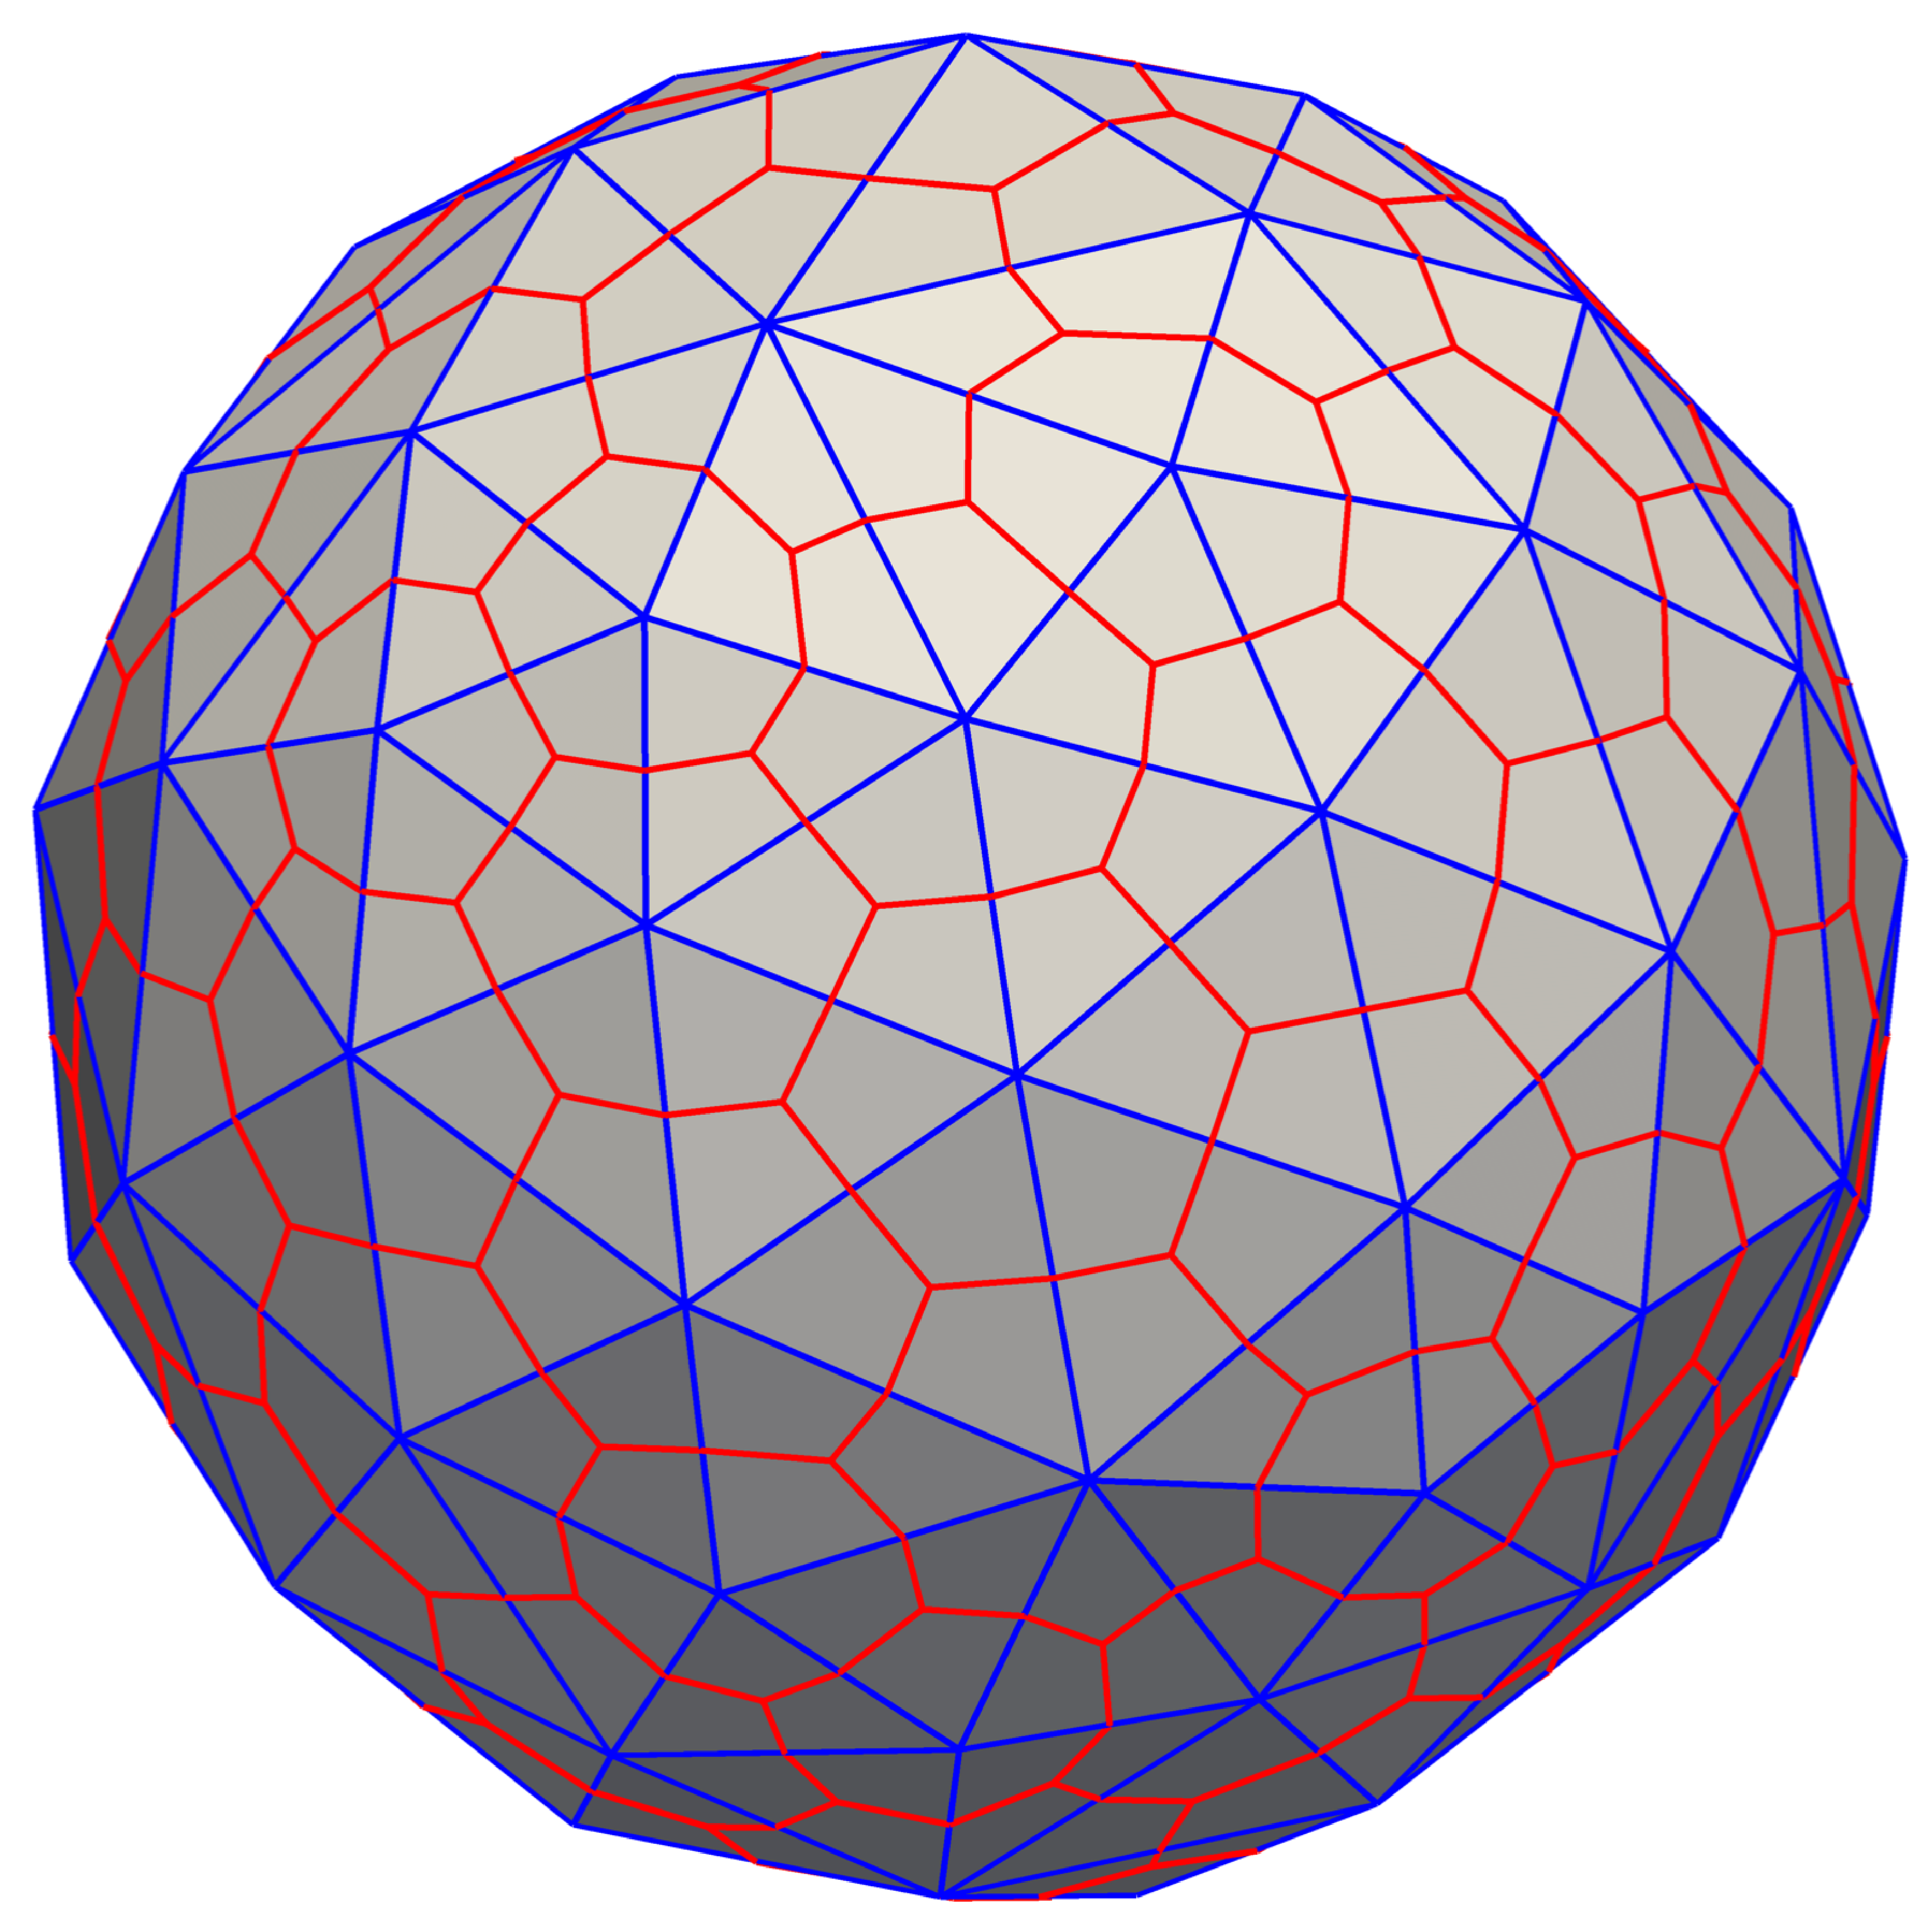
\includegraphics[width=0.6\textwidth]{img/sphere_primal_dual.pdf}
    \caption{Maillages $\ensprimalplat$ (bleu) et $\ensdualplat$ (rouge) d'une approximation polyédrique de la sphère}
\end{subfigure}%
\begin{subfigure}[t]{.5\textwidth}
    \centering
    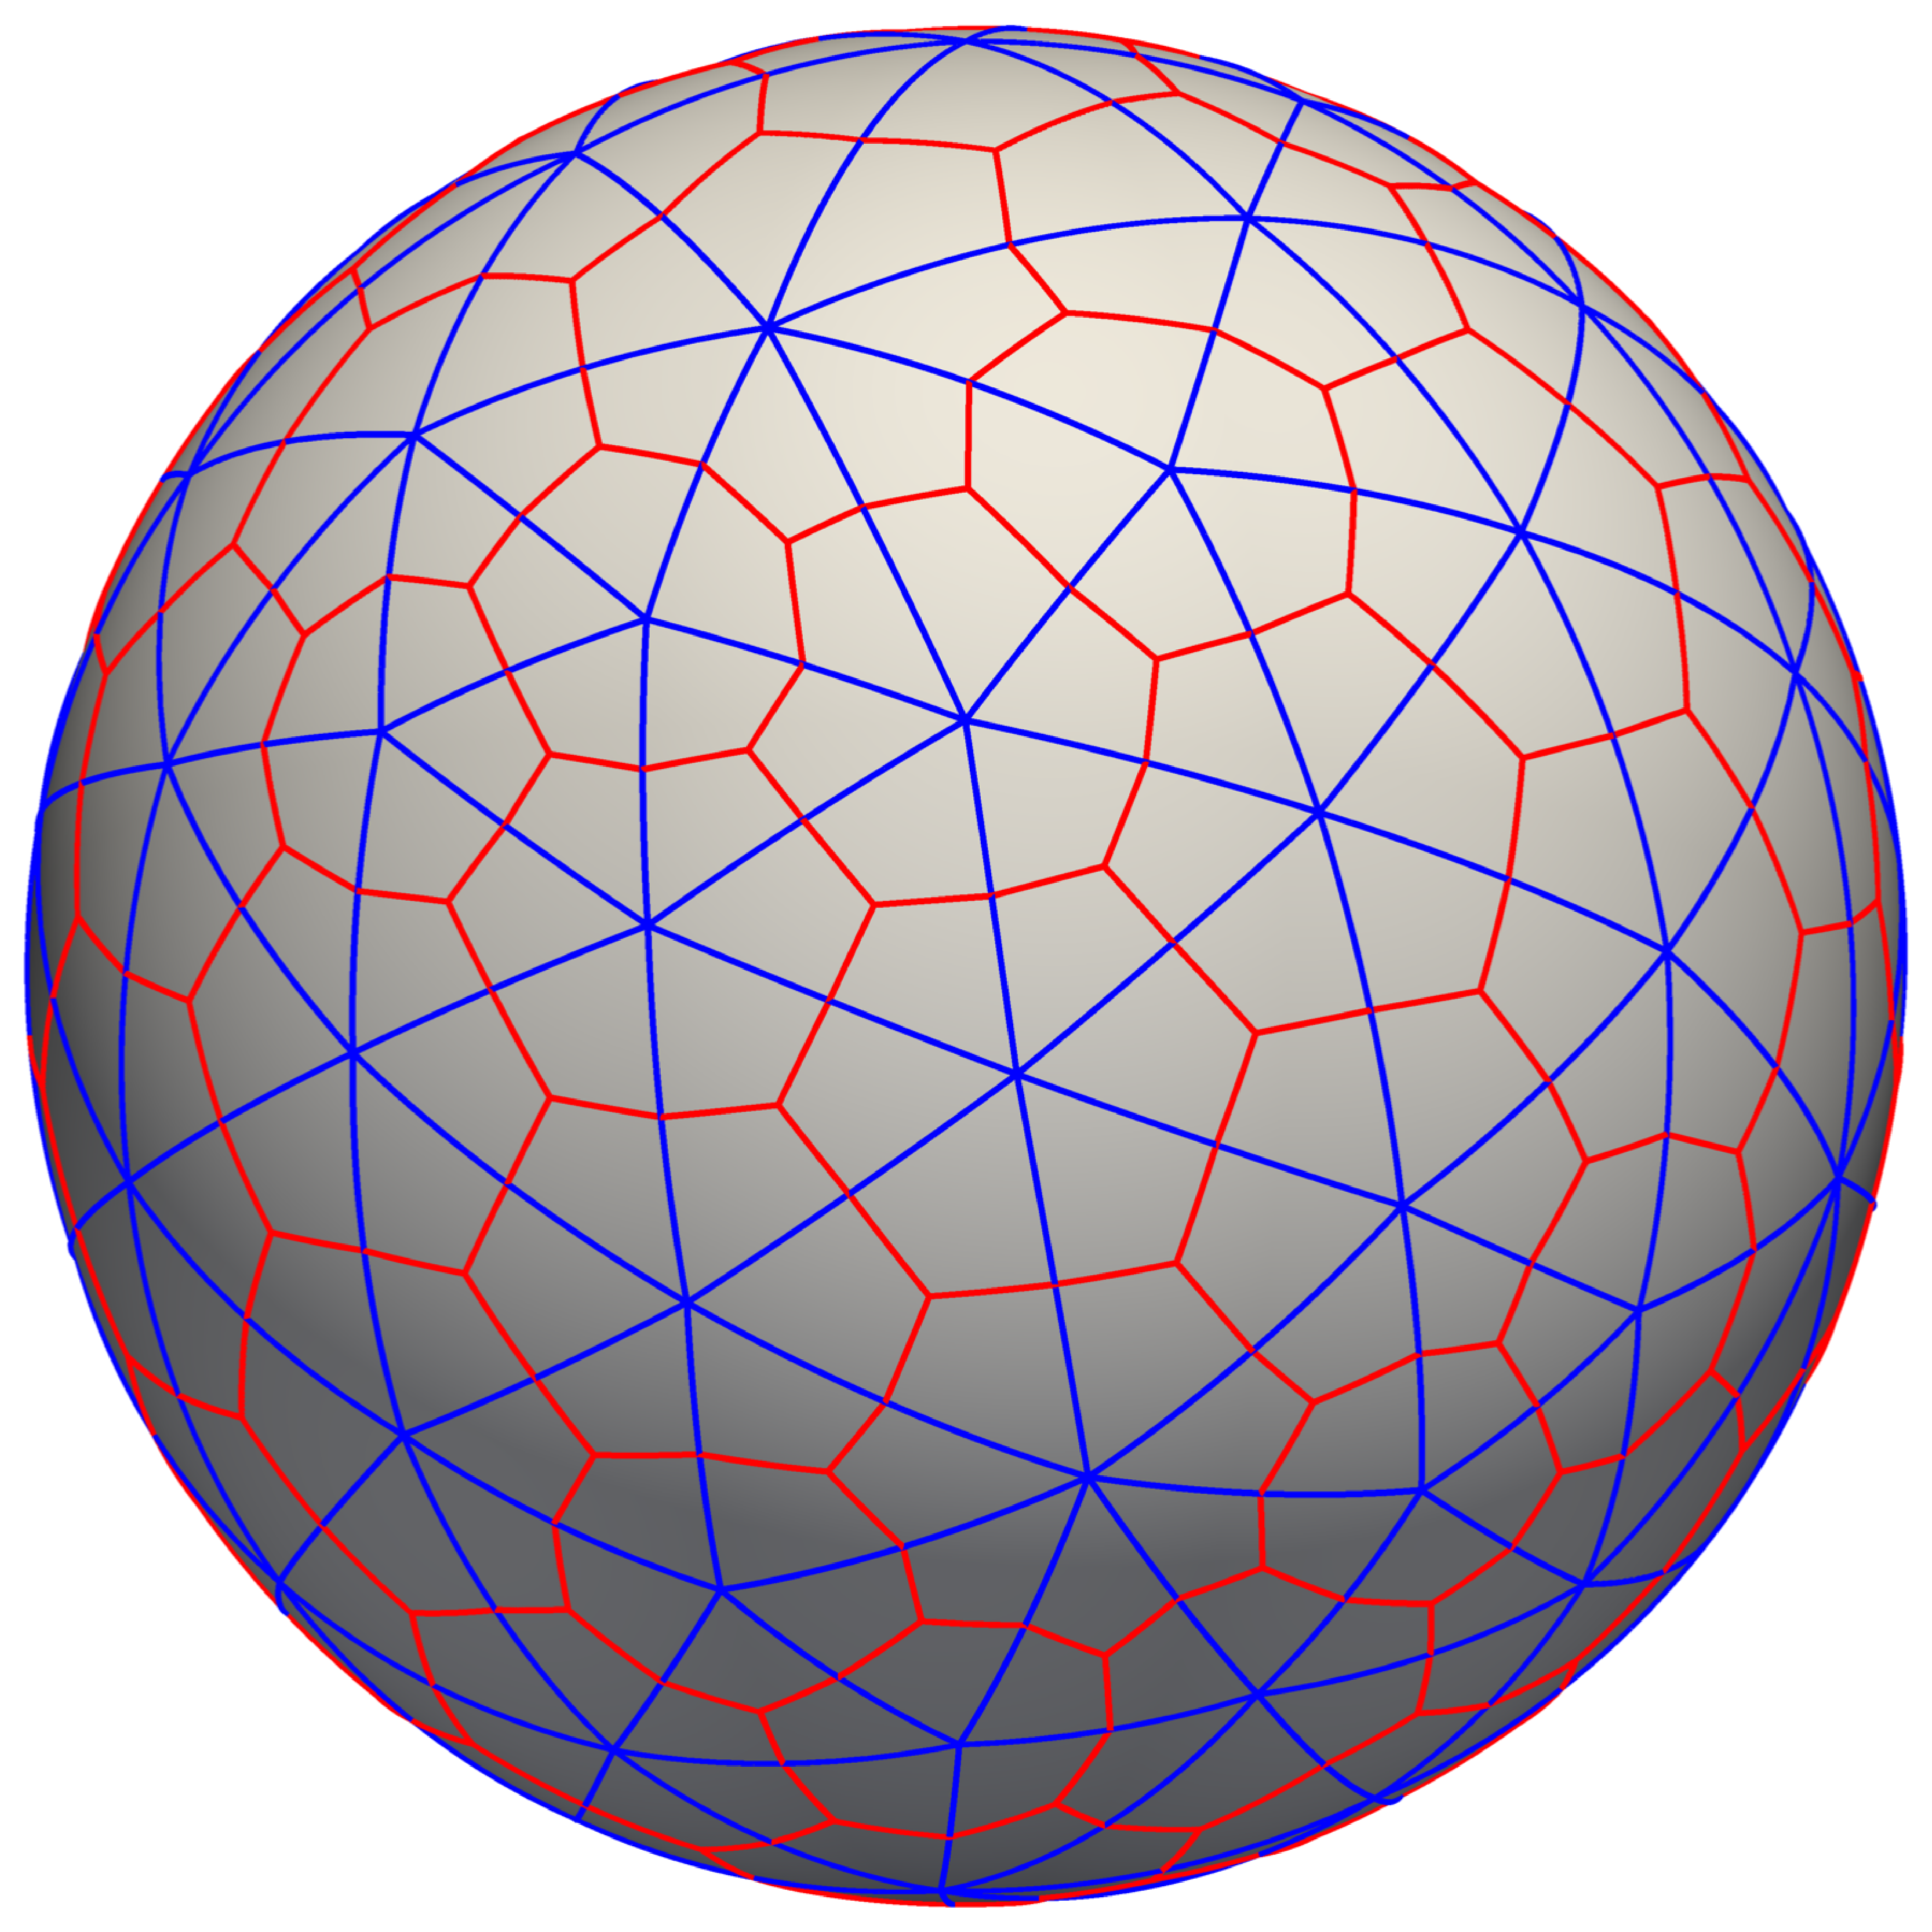
\includegraphics[width=0.6\textwidth]{img/sphere_primal_dual_curved.pdf}
    \caption{Maillages $\ensprimal$ (bleu) et $\ensdual$ (rouge) de la sphère}
\end{subfigure}
\caption{Exemple de maillages \ddfv \emph{primaux} et \emph{duaux} pour la sphère}
\end{figure}

\begin{figure}[H]
\centering
\begin{subfigure}[t]{.5\textwidth}
    \centering
    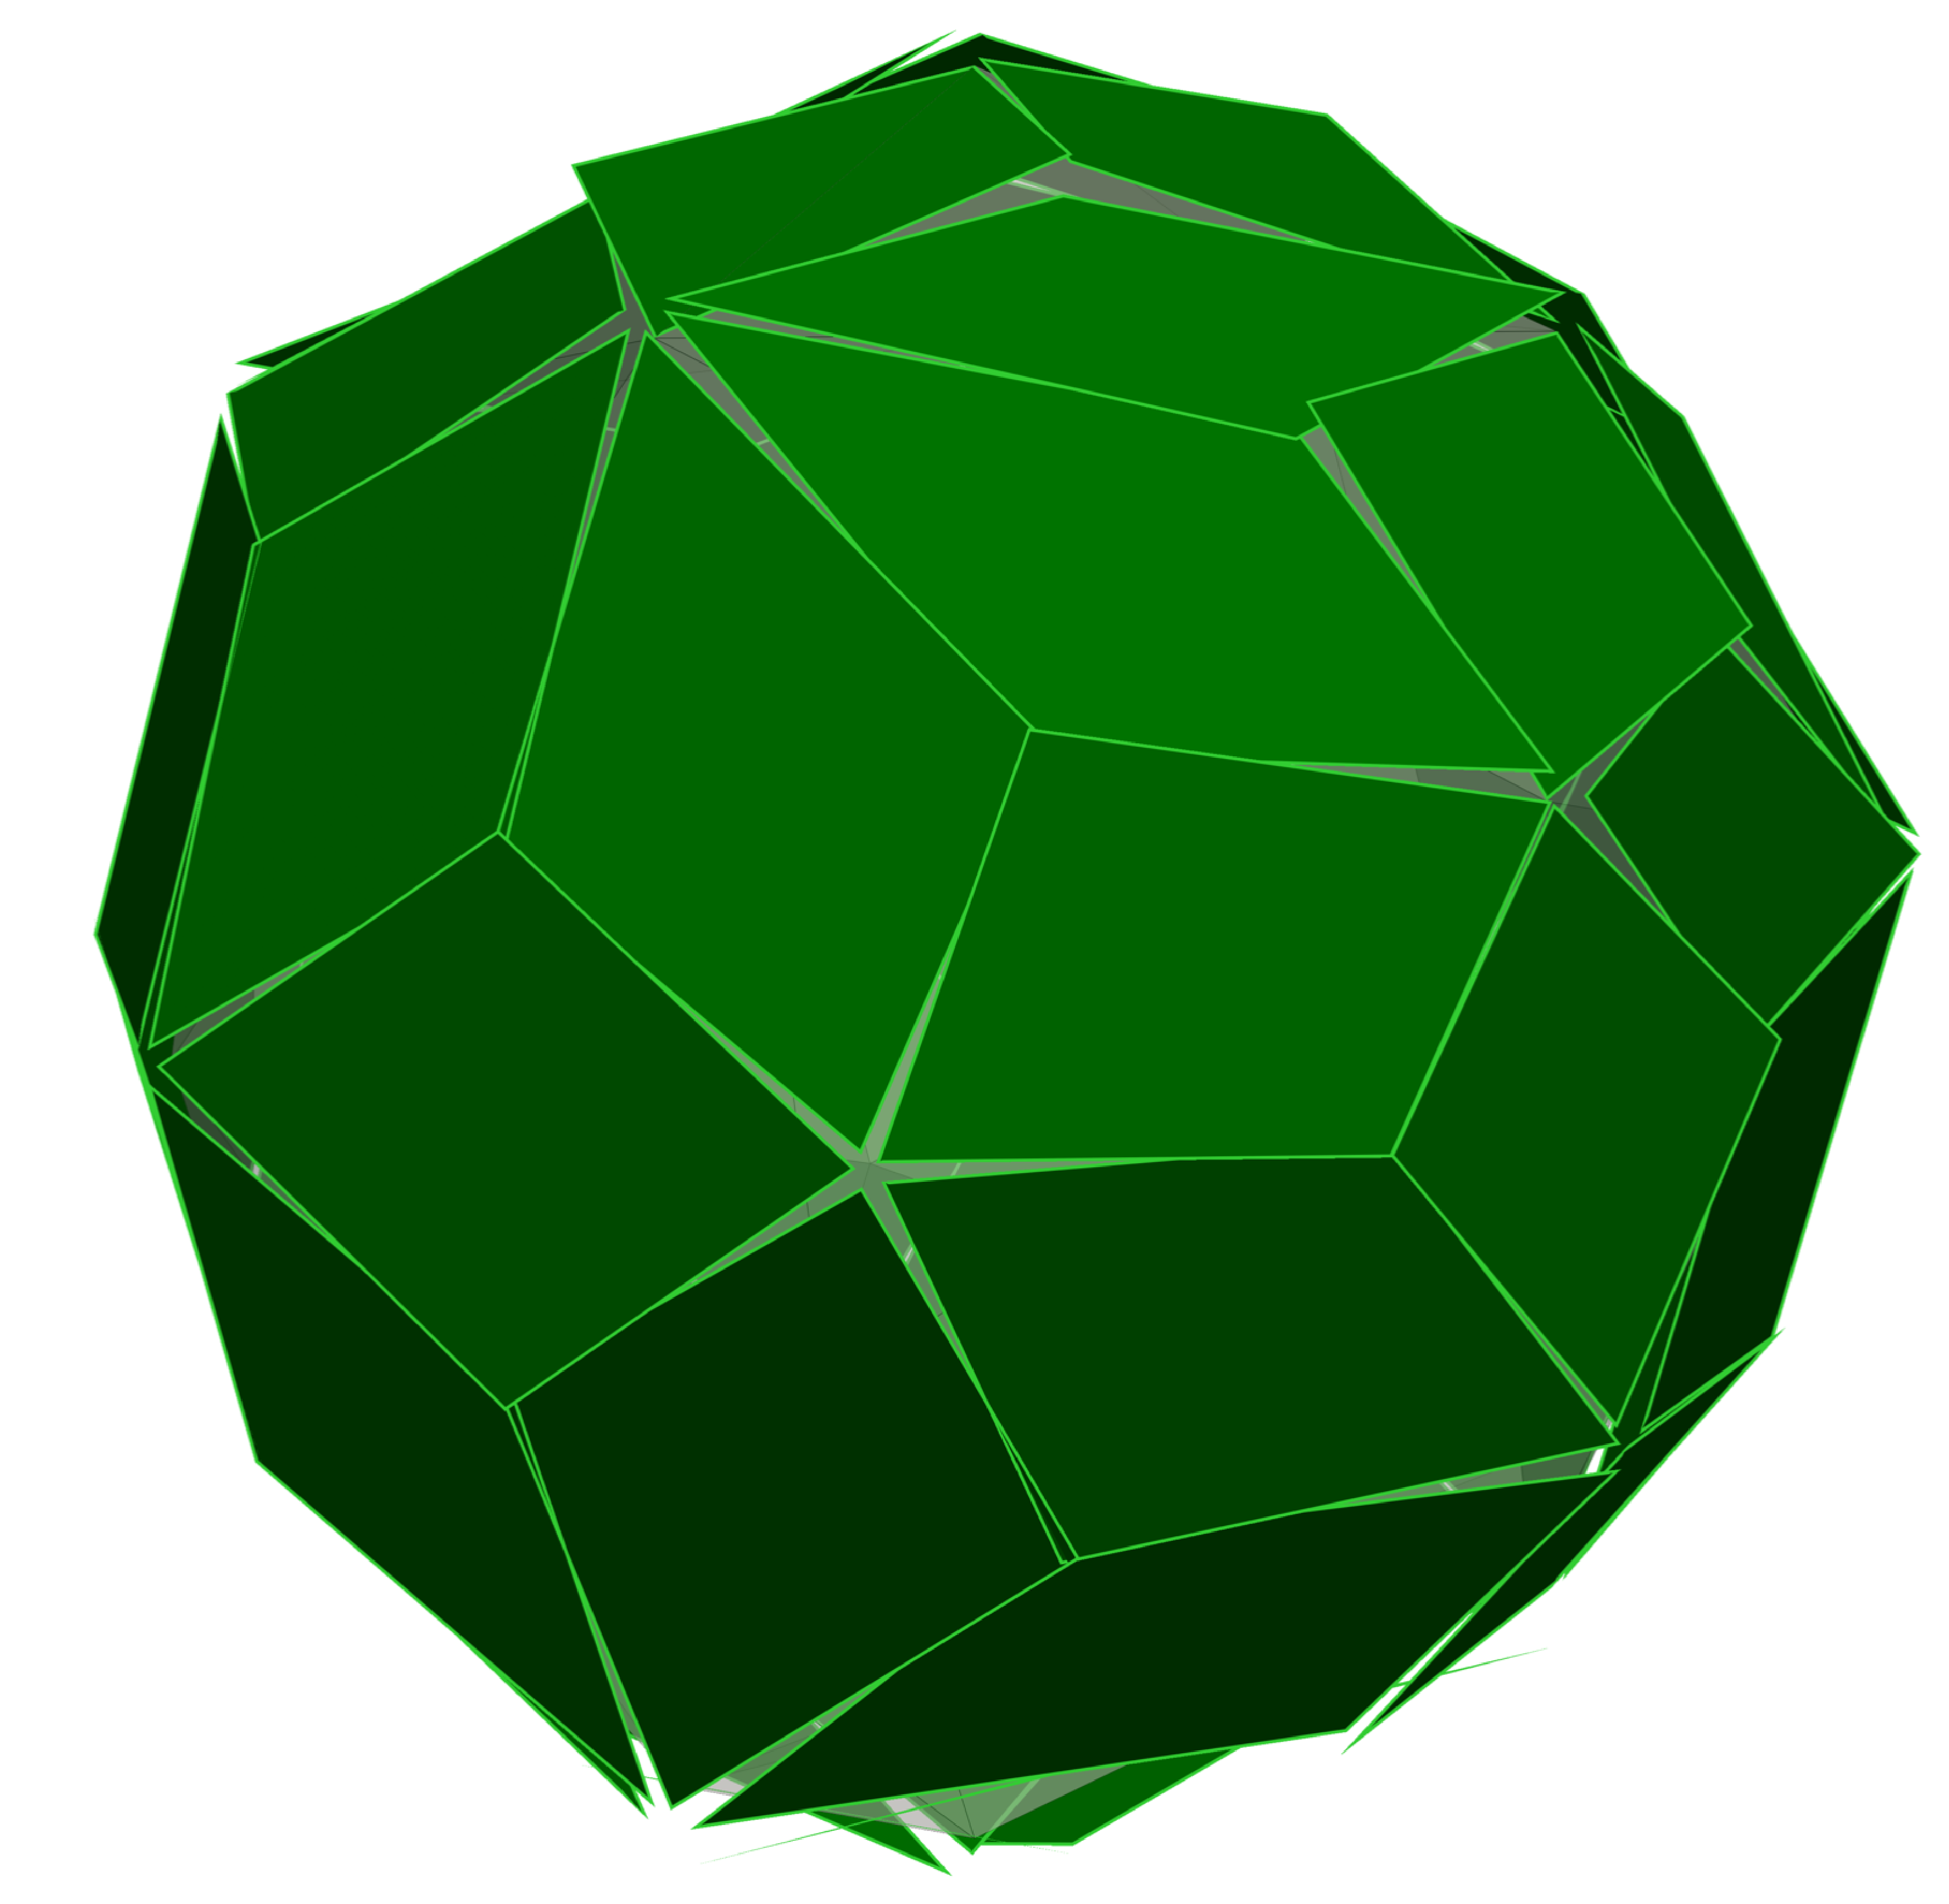
\includegraphics[width=0.6\textwidth]{img/sphere_diamonds_flat.pdf}
    \caption{Ensemble $\ensdiamantplat$}
\end{subfigure}%
\begin{subfigure}[t]{.5\textwidth}
    \centering
    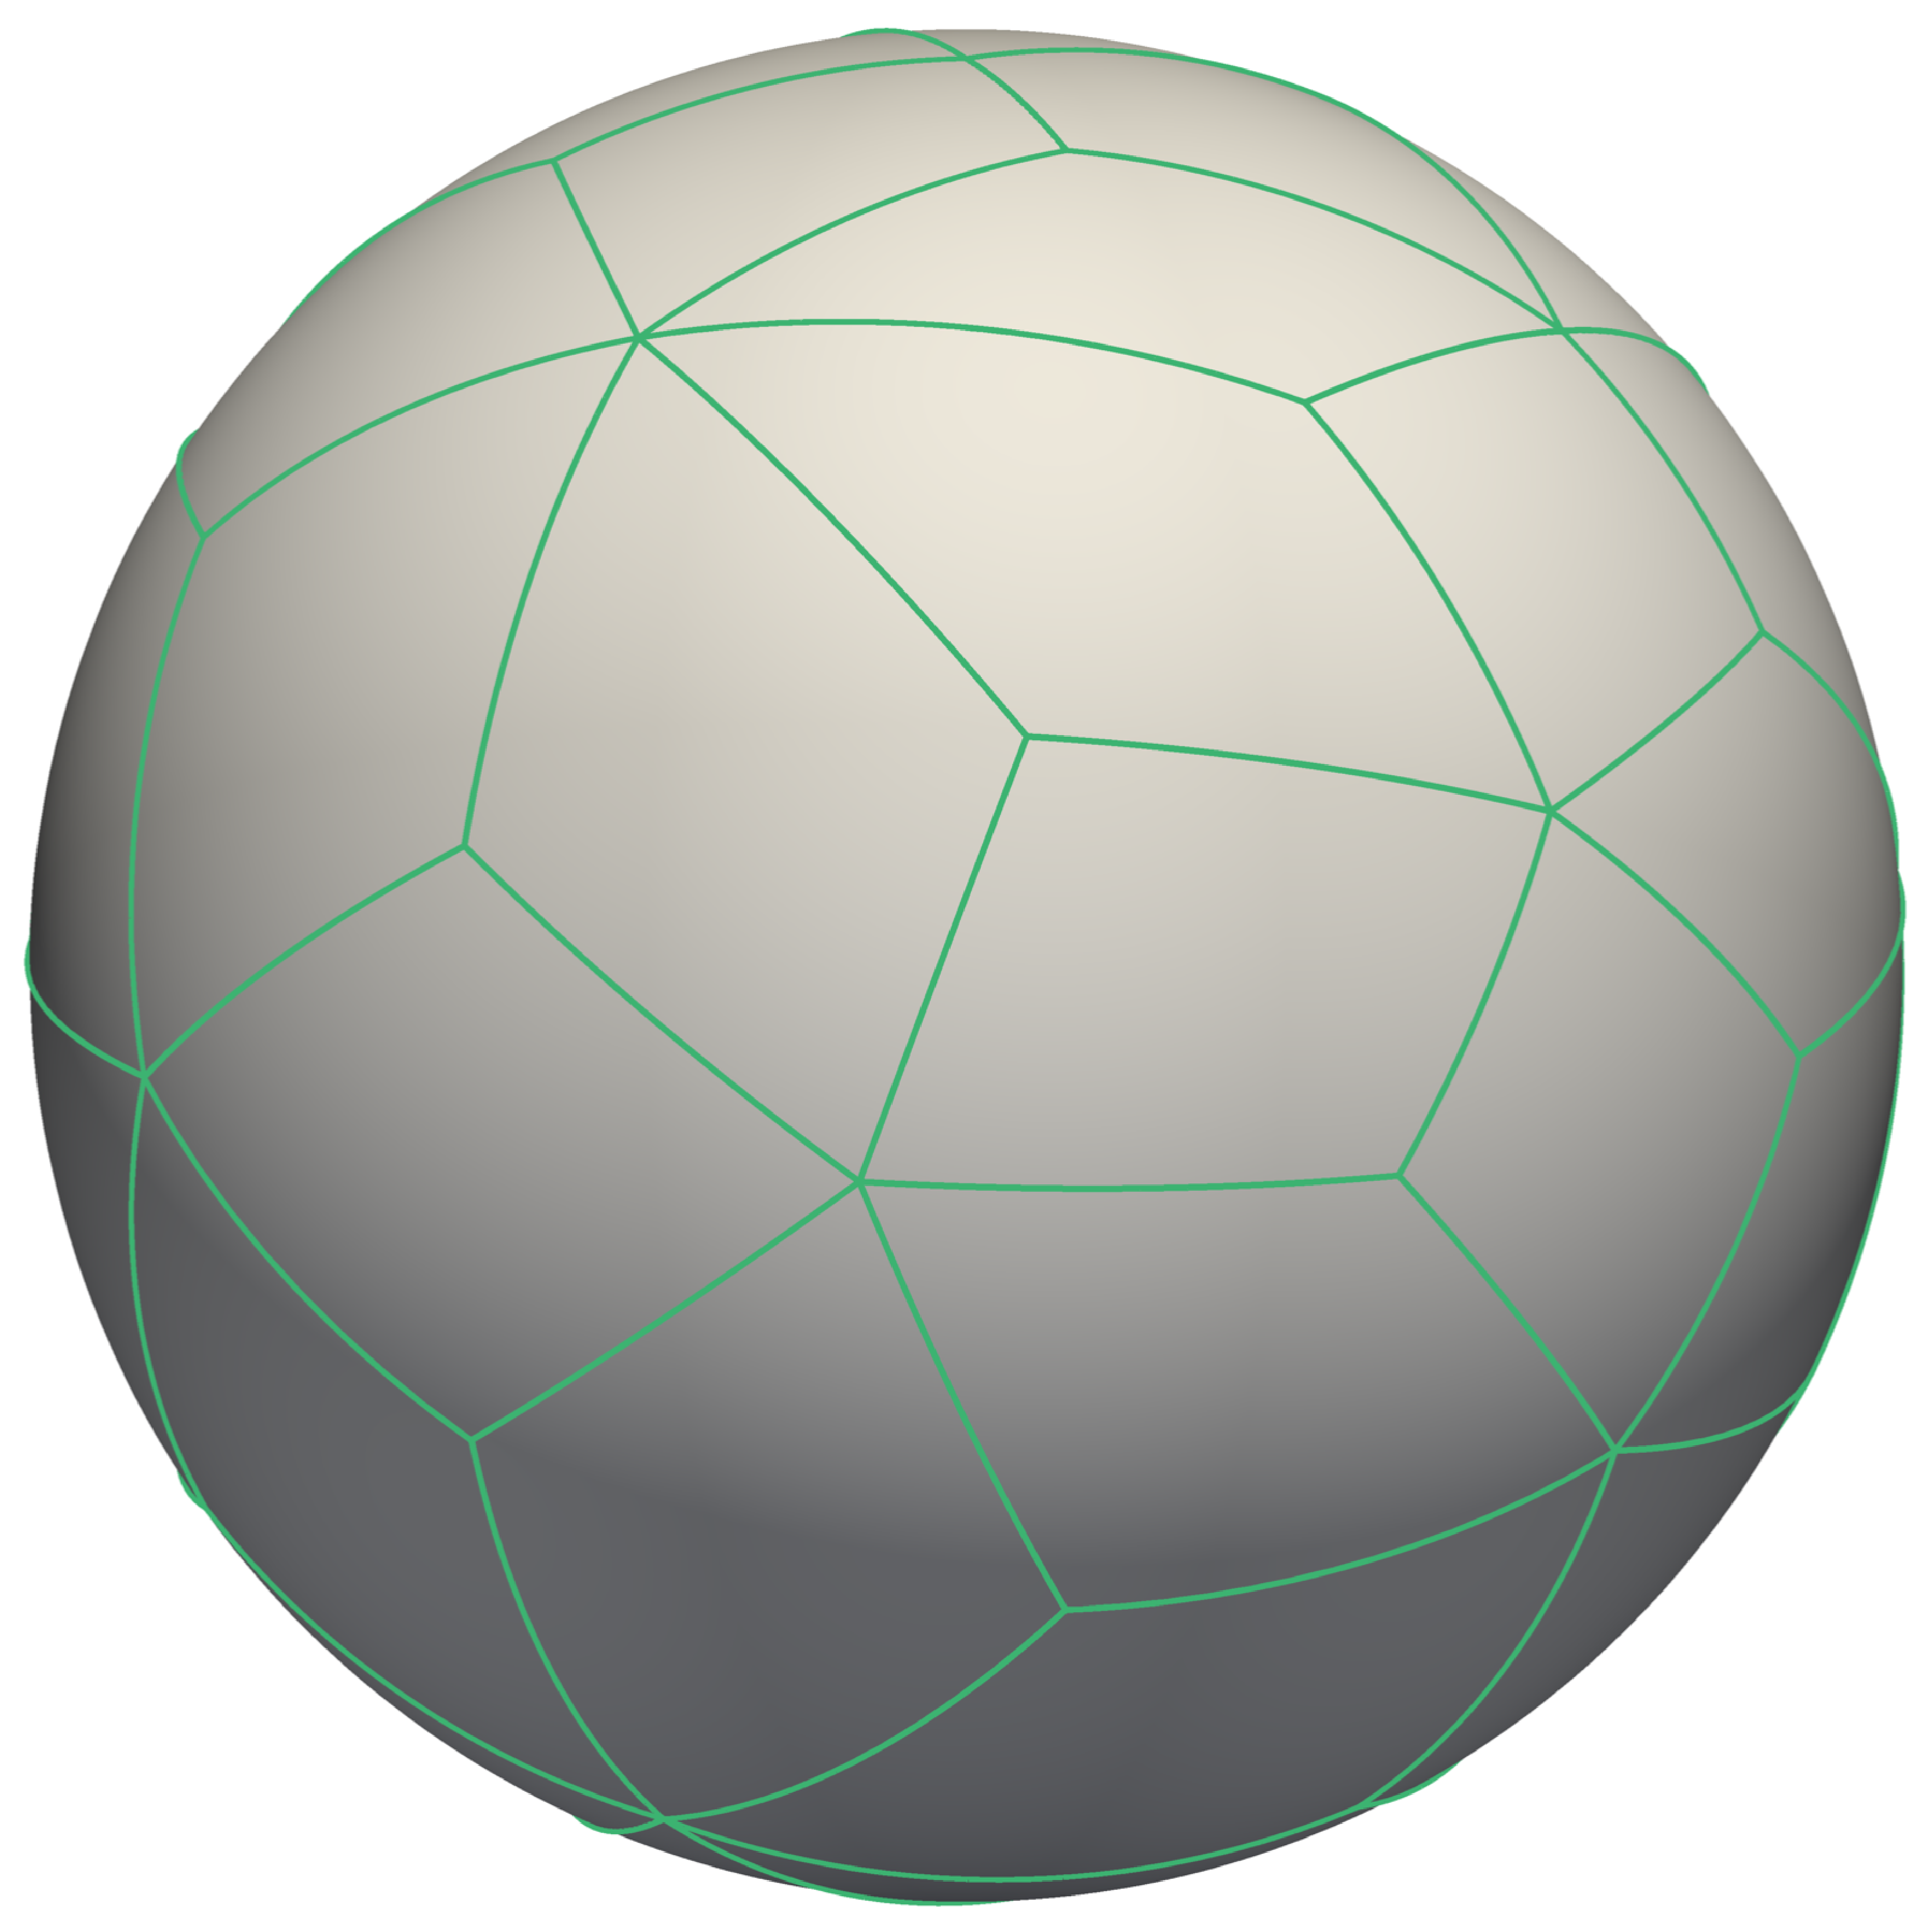
\includegraphics[width=0.6\textwidth]{img/sphere_diamond_curved_bis.pdf}
    \caption{Maillage $\ensdiamant$ de la sphère}
\end{subfigure}
\caption{Exemple de l'ensemble des diamants plats $\ensdiamantplat$ d'une discrétisation \ddfv de la sphère et du maillage \emph{diamant courbe} $\ensdiamant$ associé}
\end{figure}

\begin{figure}[H]
\centering
\begin{subfigure}[t]{.5\textwidth}
    \centering
    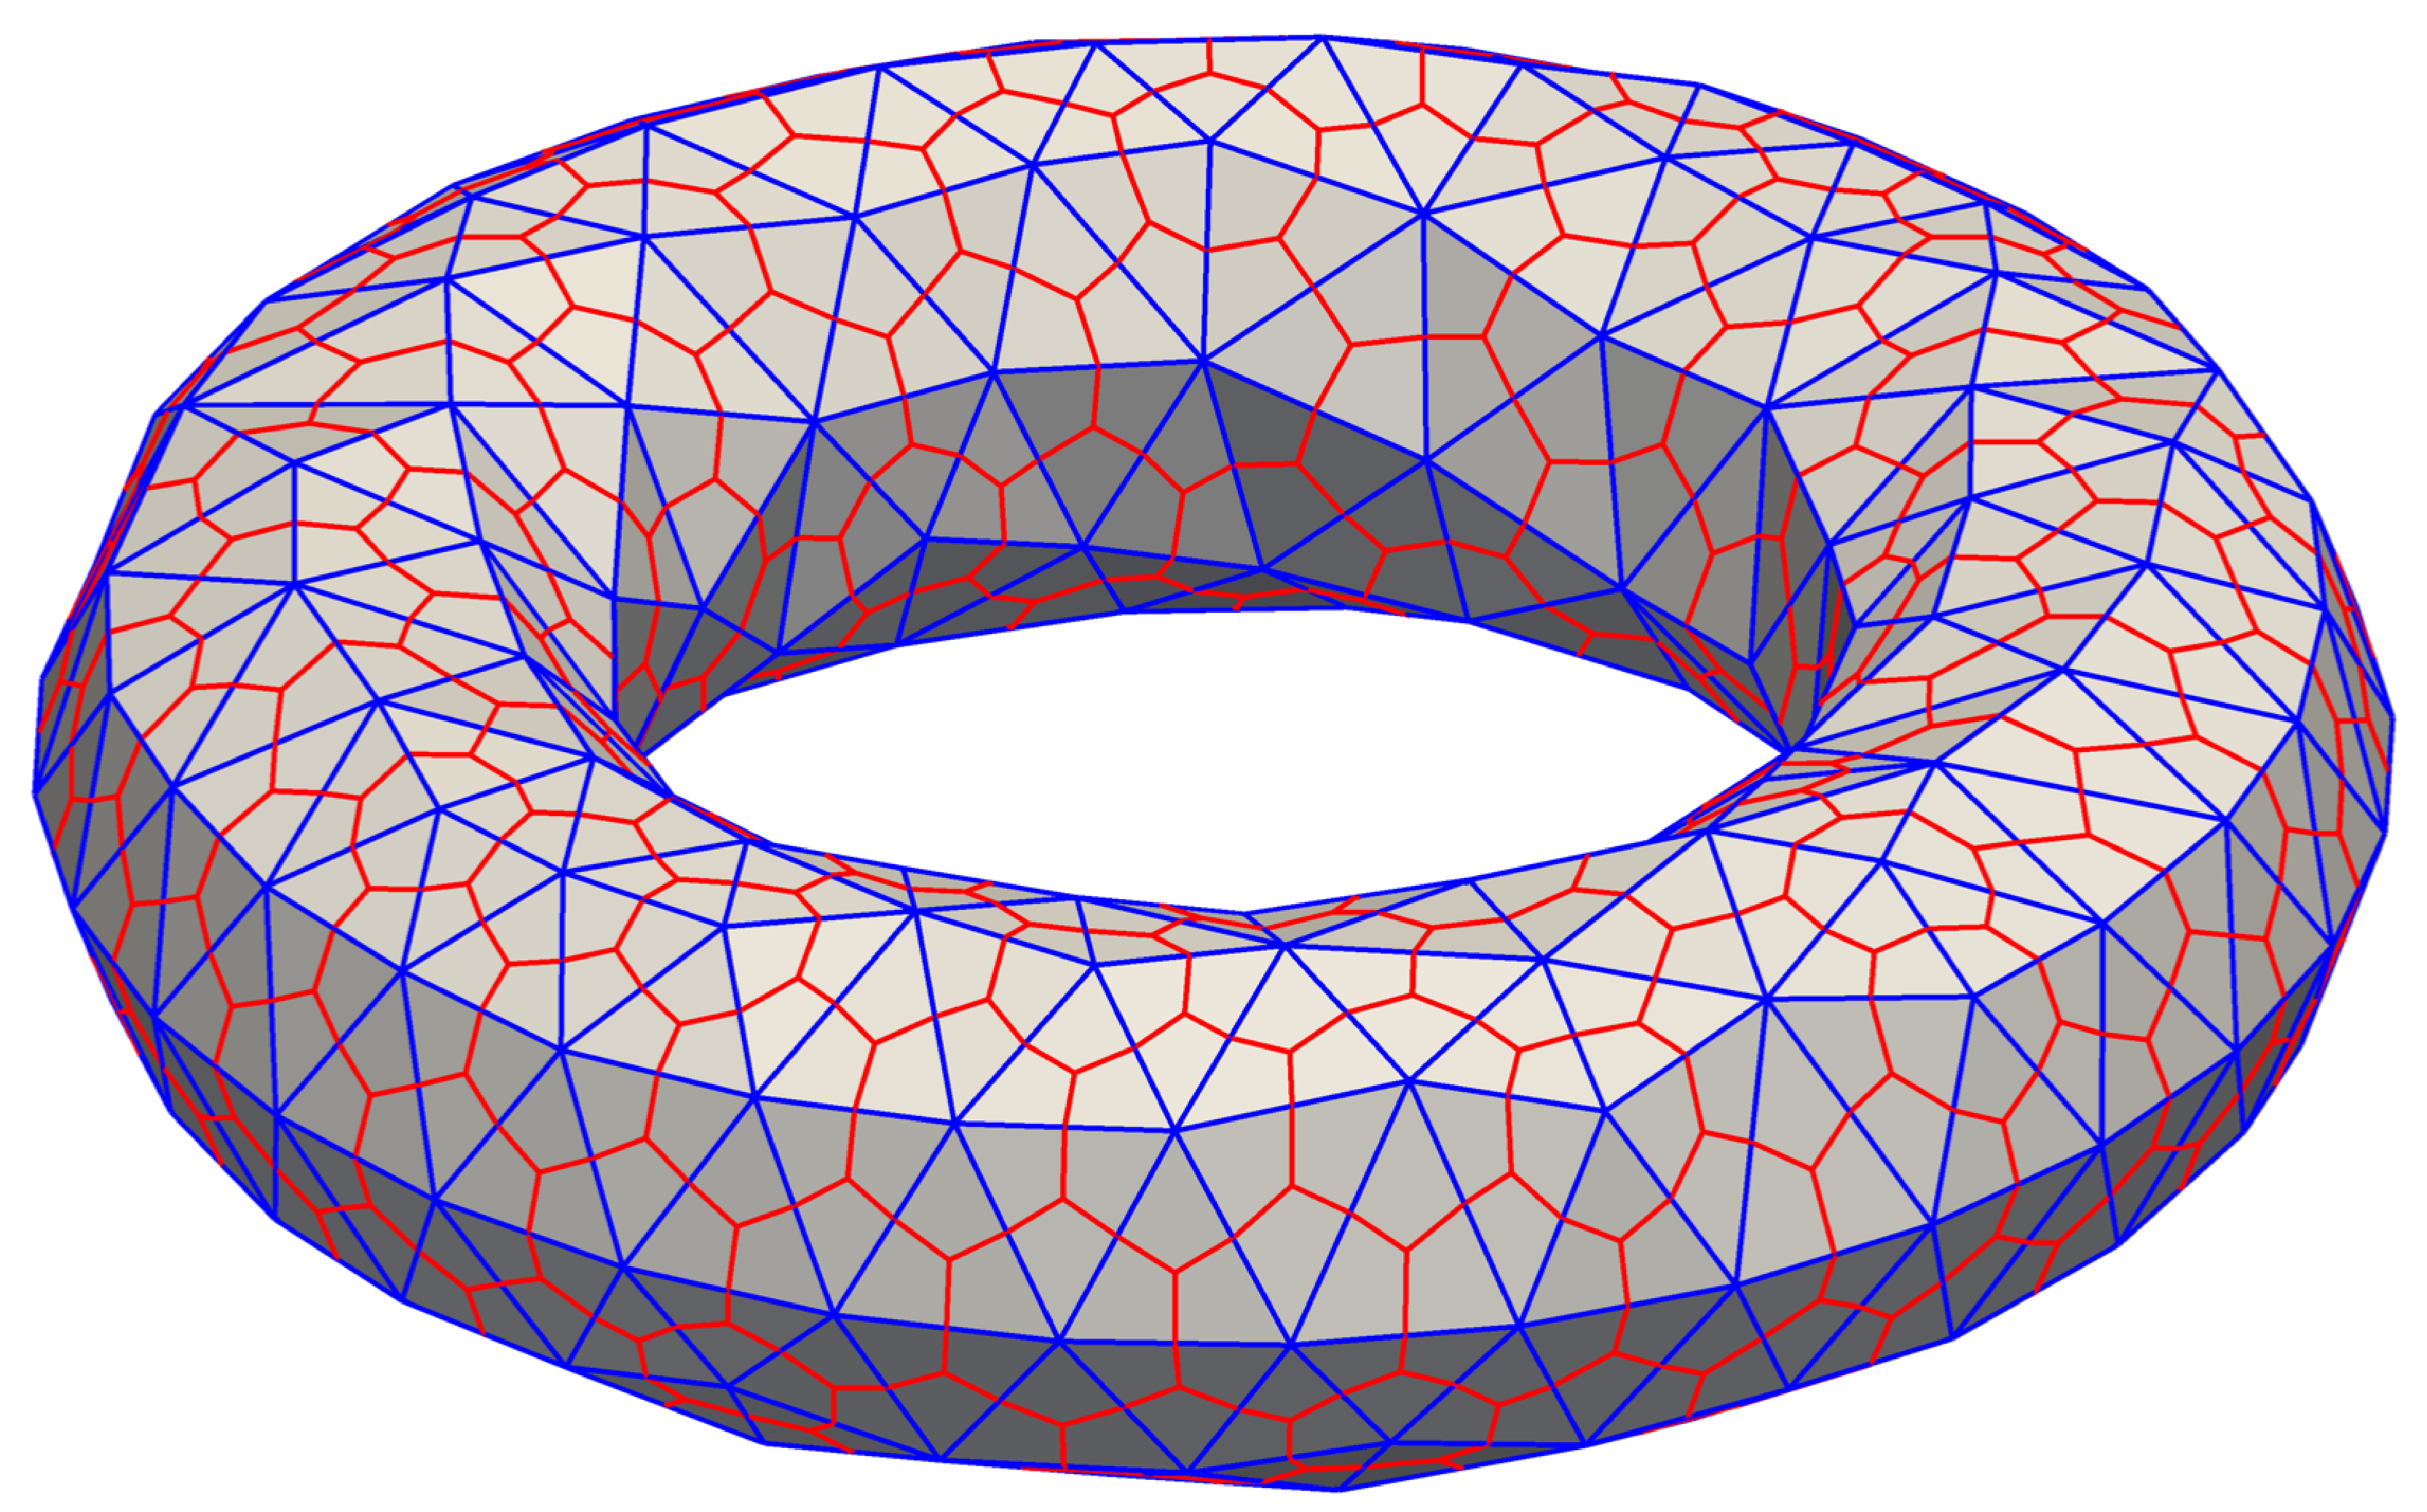
\includegraphics[width=0.7\textwidth]{img/torus_primal_dual.pdf}
    \caption{Tore, $g = 1$}
\end{subfigure}%
\begin{subfigure}[t]{.5\textwidth}
    \centering
    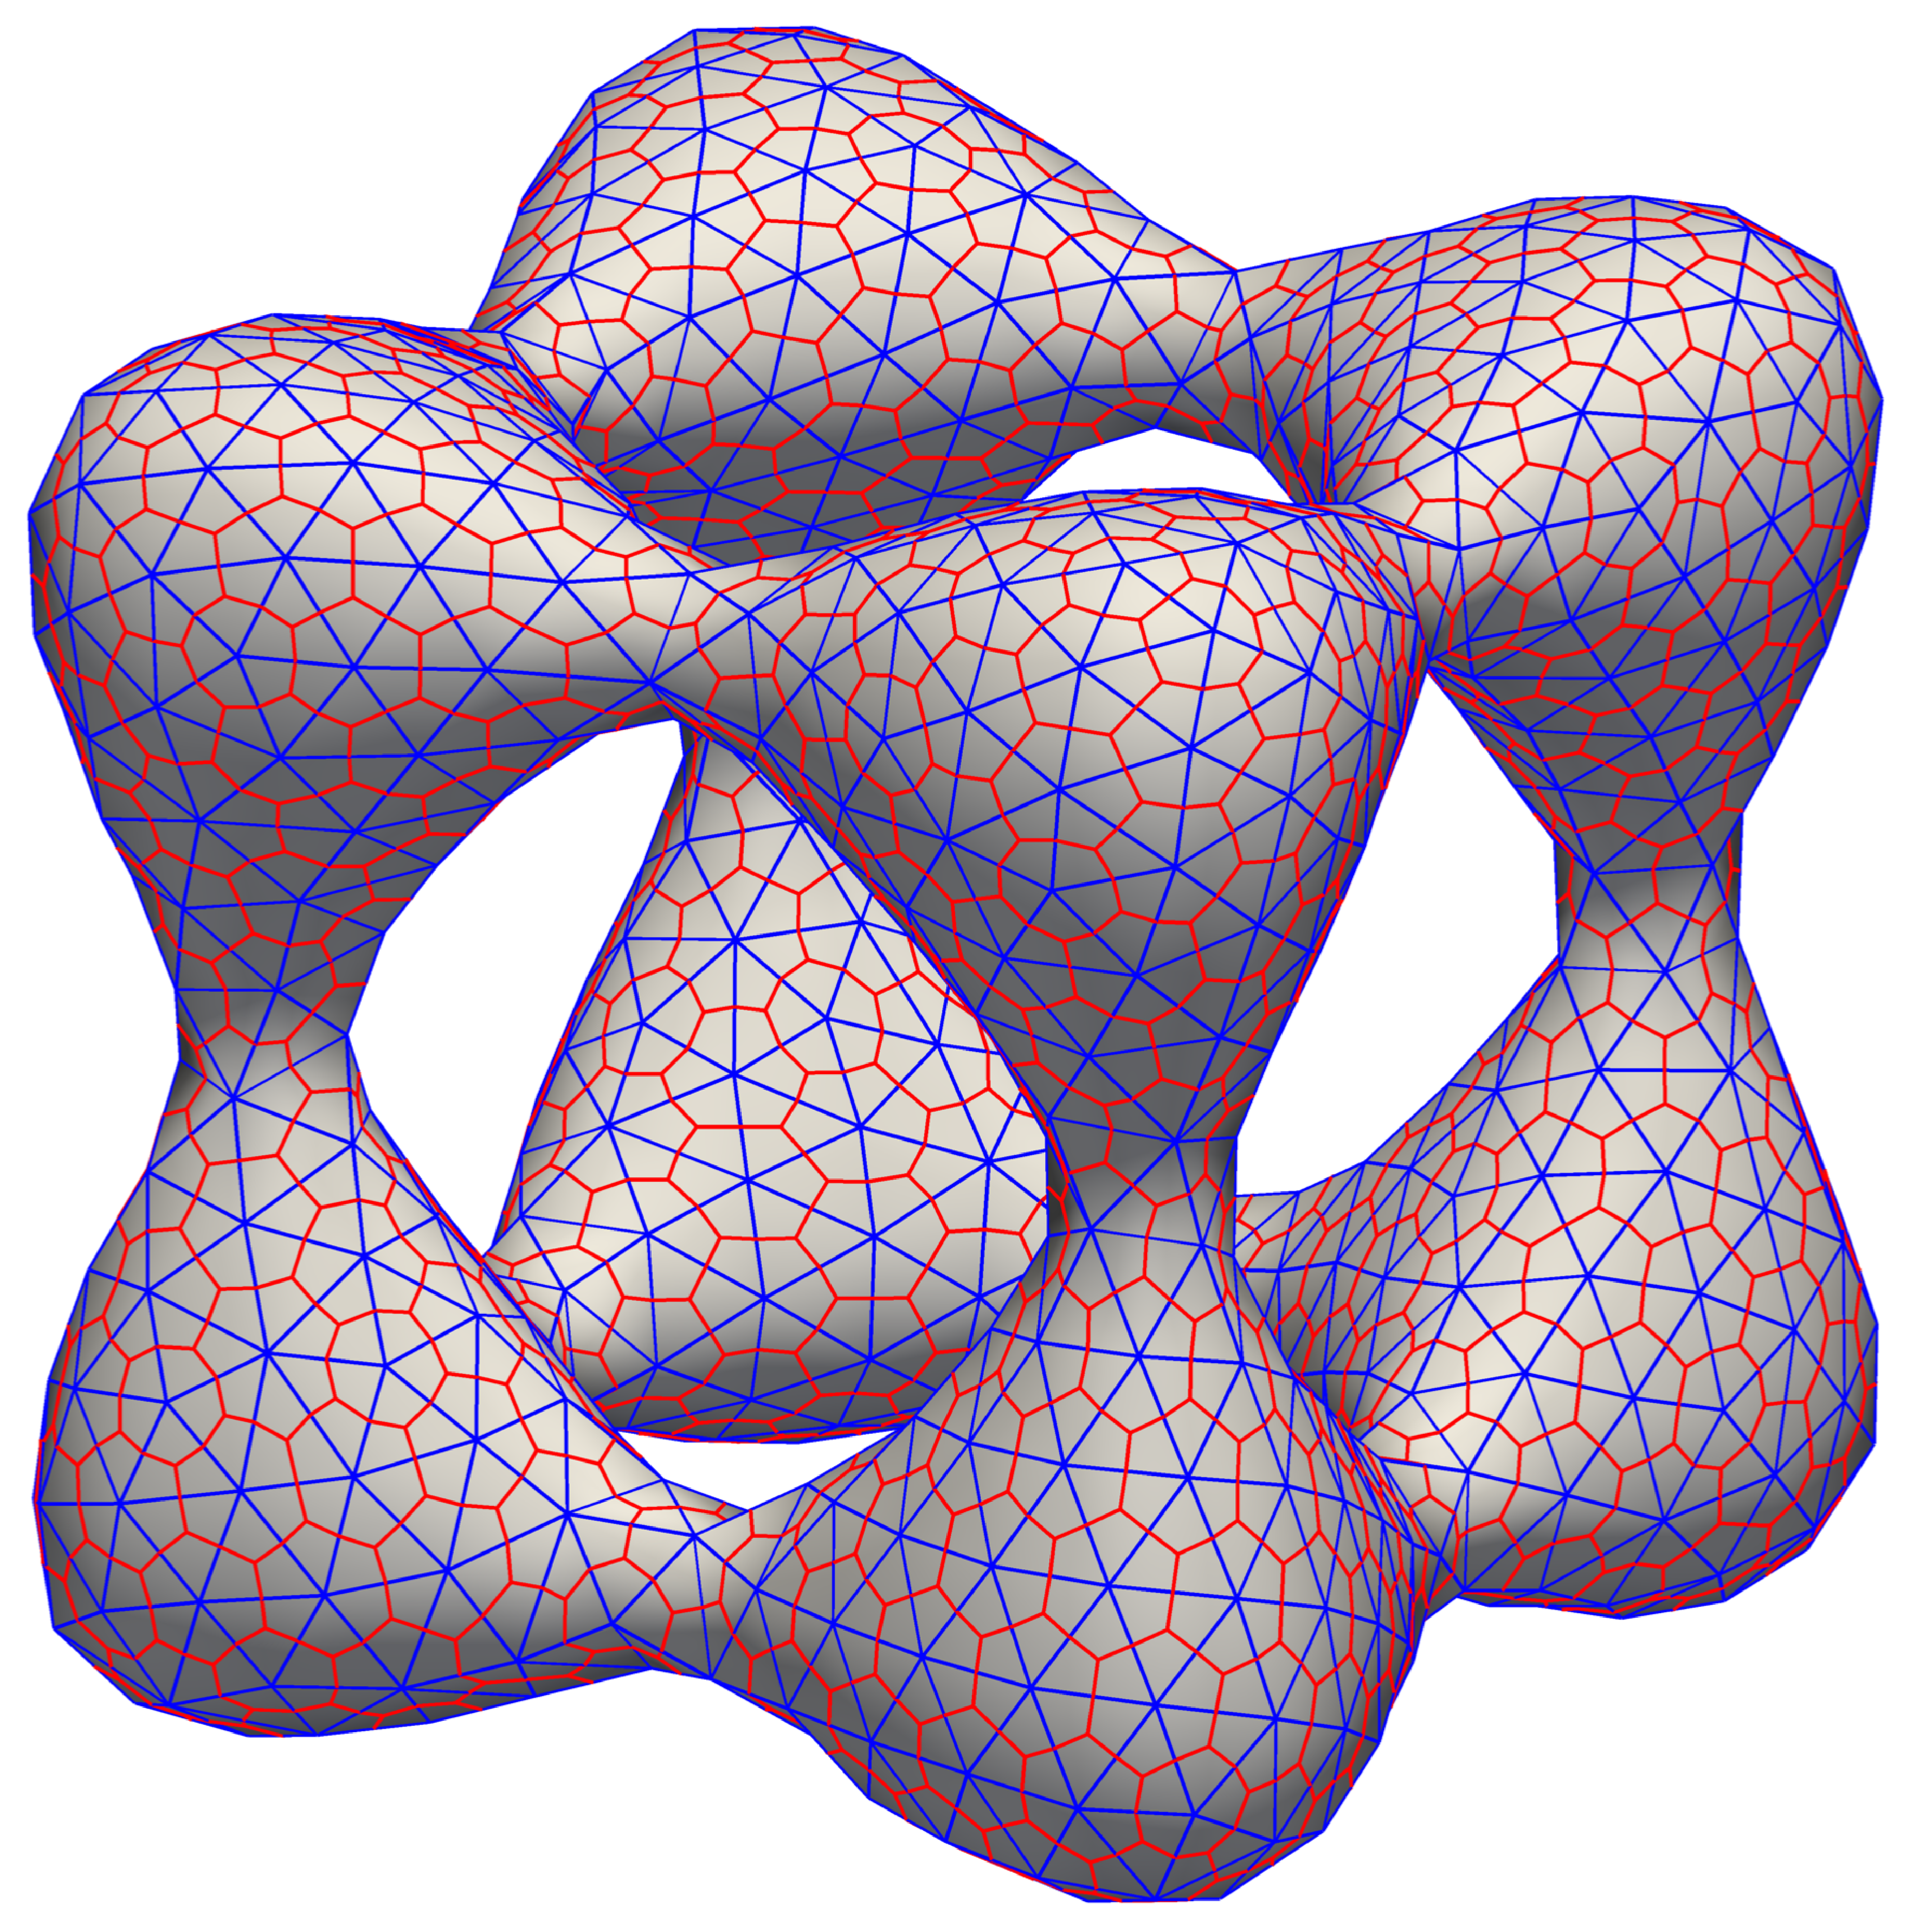
\includegraphics[width=0.6\textwidth]{img/tanglecube_primal_dual.pdf}
    \caption{\emph{Tanglecube}\protect\footnotemark, $g = 5$}
\end{subfigure}
\caption{Exemples de maillages $\ensprimalplat$ et $\ensdualplat$ sur des approximations polyédriques de surfaces fermées sans bord de $\R^3$ de genre $g > 0$}
\end{figure}
\footnotetext{Surface de degré $4$ dans $\R^3$ définie par l'équation $x^4 - 5 \, x^2 + y^4 - 5 \, y^2 + z^4 - 5 \, z^2 + 11{,}8 = 0$ (voir \url{https://academicweb.nd.edu/~jhauenst/preprints/bhrPolyTop.pdf}).}